% !TEX root=./chap-02-dummy.tex

\chapter{基于对电子方法的双杂化能量泛函实现与测评}

\section{引言}

分子体系的基态能量始终是计算化学所关心的根本问题。只有准确地描述分子基态能量,才有可能准确描述分子自由能等热力学性质,并进而将计算结果应用于反应动力学、分子动力学、精细光谱等各种具体的化学或物理问题。目前主流的对分子体系基态性质描述的理论体系,有 post-HF、DFT、QMC 等。由于 DFT 的近似方法相比于其它理论框架下的方法而言,在相同的计算资源消耗下,可以对更大的分子体系作计算、并有更高的精度,即计算消耗与精度的性价比高;因此,密度泛函近似在计算化学应用受到广泛的欢迎与使用。在第一章绪论中,也回顾到密度泛函近似的其中一个分支,双杂化泛函,在涉及主族化学的各类反应能量、弱相互作用、几何结构、分子振动与谱学问题有良好的表现。

但密度泛函近似仍然存在一些困难。目前主流的密度泛函可以依据开发模式分为两类:经验参数拟合的、与纯理论模型的。一般来说,纯理论模型的泛函在测评数据集上的表现通常稍逊色\cite{Goerigk-Grimme.PCCP.2017};但对于经验参数拟合的泛函,可能在拟合范围外产生比较严重误差,即可泛化性通常较差\cite{Medvedev-Lyssenko.S.2017}。目前流行的大多数双杂化泛函,为保证一定的泛化能力,可以采用的策略是使用较少的参数数量,如 XYG$n$\cite{Zhang-Xu.JPCL.2021} 或 DSD 系列\cite{Kozuch-Martin.JCC.2013}等泛函;或者采用复杂的参数拟合策略,如 ωB97X-2\cite{Chai-Head-Gordon.JCP.2009} 或 ωB97M(2)\cite{Mardirossian-Head-Gordon.JCP.2018}等泛函。这些泛函的参数通常是针对主族化学体系的反应能与弱相互作用能数据集上拟合得到;但目前的测评中,这些泛函确实在原子密度\cite{Su-Xu.PNAS.2018}、偶极矩与极化率\cite{Hait-Head-Gordon.JCTC.2018, Hait-Head-Gordon.PCCP.2018}、化学位移\cite{Stoychev-Neese.JCTC.2018}等问题上有良好的结果,即表现出不错的泛化能力。但同时需要注意到,这些泛函仍然在以过渡金属为代表的一些计算问题上,数值表现通常还有提升的空间。

目前流行的双杂化泛函中,通常引入了 MP2 型相关能 $E_\mathrm{c}^\mathrm{MP2}$。若分子体系的 HOMO/LUMO gap 较小,则 $E_\mathrm{c}^\mathrm{MP2}$ 会产生严重的负误差。由于一部分过渡金属与多参考问题具有 HOMO/LUMO gap 较小的特性,因此双杂化泛函在这类问题上表现较差。波函数理论中,与 MP2 计算量相仿的电子对方法 IEPA\cite{Sinanoǧlu-Sinanoǧlu.ACP.1964, Nesbet-Nesbet.ACP.1965}、sIEPA\cite{Zhang-Scheffler.PRL.2016}、MP2/cr\cite{Dykstra-Davidson.IJQC.2000}\footnote{在 Dykstra and Davidson 原文\cite{Dykstra-Davidson.IJQC.2000}中提出了两种 MP2/cr 形式。原文的 MP2/cr-II 的计算需要自旋相同且同占据轨道角标的激发系数 $t_{i \bar i}^{a \bar b}$;这在 $\alpha, \beta$ 占据数不同的情形下难以合理地定义。在正文中,我们仅介绍与使用原文的 MP2/cr-I,并将其指代为 MP2/cr。} 等可以一定程度地避免 $E_\mathrm{c}^\mathrm{MP2}$ 型相关能的负误差。在双杂化泛函中引入这类相关能,有望在不加大计算量的同时,提高 HOMO/LUMO gap 较小体系问题的计算精度。这三类近似方法在本工作中统称为 IEPA 型相关能。

在理论层面,掺杂 MP2 型相关能的双杂化泛函基础,一般认为是 G\"orling-Levy 微扰理论的二阶近似。事实上,G\"orling-Levy 微扰理论建立起了密度泛函方法与波函数理论之间的联系,而这层联系不仅仅局限于二阶微扰、还可以与更高级的方法产生联系。从这个角度来看,在密度泛函中引入不同于 MP2 的其它波函数理论下的相关能,在 G\"orling-Levy 微扰理论的角度下是可以立足的。

基于这些认识,在本章工作中,将实现掺杂 IEPA 型相关能的双杂化泛函,并进行理论合理性说明与测评。\ref{sec.2.iepa-gl-perturb} 节将回顾 G\"orling-Levy 微扰理论,进一步详细地阐述其与波函数理论之间的关系,以及在密度泛函近似中引入波函数方法相关能的合理性。\ref{sec.2.iepa-theory} 节将回顾作为波函数理论的 IEPA 型相关能近似理论与计算实现。\ref{sec.2.iepa-results} 节将通过参数拟合的方式给出掺杂 IEPA 型相关能的双杂化泛函,并对部分主族化学、过渡金属体系、多参考问题进行测评,以及对参数优化过程进行讨论。

\section{理论背景:密度泛函方法}
\label{sec.2.iepa-gl-perturb}

\subsection{绝热路径与耦合系数}

波函数理论下的 post-HF 理论可以在 CI、CC 等理论框架下,通过引入更多的多电子波函数,以更大代价、但切实有效地逼近真实能量。不同于波函数理论近似,密度泛函近似发展的困难之一,在于难以找到一条逼近真实泛函的路径。绝热路径理论联系起波函数理论与密度泛函理论两者。一方面,通过借鉴与引入波函数理论的一些内容,可以进一步发展密度泛函理论;另一方面,绝热路径也提供了一种路径,使得数值上逼近真实泛函成为可能。

考虑下述关于耦合常数 $\lambda$ (coupling constant) 与有效势 $v(\bm{r})$\footnote{这一小节中,$v(\bm{r})$ 记号不表示体系外势,而是任意势函数。这与绪论的行文有记号上的冲突。外势函数在这记为 $v_\mathrm{ext} (\bm{r})$。} 的算符 $\hat H_\lambda [v]$: 
\begin{equation}
  \label{eq.2.H-lambda}
  \hat H_\lambda [v] = \hat T + \lambda \hat V_\mathrm{ee} + \sum_i^{n_\mathrm{elec}} v(\bm{r}_i)
\end{equation}
定义下述关于耦合常数 $\lambda$ 与有效势 $v(\bm{r})$ 的能量泛函\footnote{这里的许多记号不严谨,因泛函必须要在合理的函数空间下才能有定义;并且存在许多极值问题无法用最小 (min)、最大值 (max) 定义,而需要用函数收敛的上界 (sup)、下界 (inf) 定义。我们在这里通常只考虑 $N$ 可表示密度、无简并基态的情形。依据 Lieb 工作\cite{Lieb-Lieb.IJQC.1983}中定理 3.3 的证明,这类情形下许多下界可以取到最小、上界可以取到最大;且由于不考虑简并情况,泛函最小、最大值及其对应的自变量都是唯一的。}
\begin{equation}
  \label{eq.2.E-lambda}
  E_\lambda [v] = \min_{\Psi} \langle \Psi | \hat H_\lambda [v] | \Psi \rangle 
\end{equation}
这里我们不考虑简并的情况。我们定义在势函数 $v(\bm{r})$、耦合常数 $\lambda$ 下,波函数 $\Psi_\lambda [v]$ 为
\begin{equation}
  \label{eq.2.E-lambda-psi}
  \Psi_\lambda [v] = \arg \min_{\Psi} \langle \Psi | \hat H_\lambda [v] | \Psi \rangle
\end{equation}
作为特殊情况
\begin{itemize}[nosep]
  \item 当 $\lambda = 1$ 且 $v(\bm{r})$ 是体系外势 $v_\mathrm{ext} (\bm{r})$ 时,$E_{\lambda=1} [v_\mathrm{ext}]$ 就是体系的基态能量,$\Psi_{\lambda=1}$ 即体系的真实波函数。

  \item $\lambda = 0$ 且 $v(\bm{r})$ 为库伦势
  $$v_\mathrm{J} (\bm{r}) = \frac{\delta J[\rho]}{\delta \rho(\bm{r})}, \quad J[\rho] = \int \frac{\rho(\bm{r}) \rho(\bm{r}')}{|\bm{r} - \bm{r}'|} \, \mathrm{d} \bm{r} \, \mathrm{d} \bm{r}'$$
  交换相关势
  \begin{equation*}
    v_\mathrm{xc} (\bm{r}) = \frac{\delta E_\mathrm{xc}[\rho]}{\delta \rho(\bm{r})}, \quad E_\mathrm{xc} [\rho] = (T[\rho] - T_\mathrm{s} [\rho]) + (F_{\lambda=1} [\rho] - J[\rho])
  \end{equation*}
  与体系外势 $v_\mathrm{ext} (\bm{r})$ 之和时,$E_{\lambda=0} [v]$ 所给出的基态波函数 $\Psi_{\lambda=0}$ 对应的密度等于 $E_{\lambda=1} [v_\mathrm{ext}]$ 体系的密度\footnote{需要注意到一般地,当 $v = v_\mathrm{xc} + v_\mathrm{J} + v_\mathrm{ext}$ 时,$E_{\lambda=0} [v] \neq E_{\lambda=1} [v_\mathrm{ext}]$。即尽管 $\lambda = 0$ 与 $\lambda = 1$ 时的密度 $\rho(\bm{r})$ 相同,但对应的能量不同。}。由于 $\hat H_{\lambda=0} [v] = \hat T + \sum_{i} v(\bm{r}_i)$ 是单电子算符,因此若不考虑简并情况,其基态波函数必然可以通过行列式表达 (该情形也称为无相互作用体系)\footnote{如第一章所述,对于 $\lambda = 0$ 的情形,基态波函数 $\Psi_{\lambda = 0}$ 也可以通过占据轨道的 Hartree 连乘积的形式给出。Hartree 乘积波函数、与作为连乘积线性组合的行列式波函数,在 $\hat H_{\lambda=0} [v]$ 下的期望相等,表达的是相同的物理状态。但出于后续定义 $E_\mathrm{x}^\text{exact}$ 的便利,在此我们定义 $\Psi_{\lambda = 0}$ 为行列式。};依据 Kohn-Sham 方程的表达式,当 $v = v_\mathrm{xc} + v_\mathrm{J} + v_\mathrm{ext}$ 时,这样的行列式是通过 Kohn-Sham 轨道构成的。
\end{itemize}
因此可以说从概念上,泛函 $E_\lambda [v]$ 通过耦合常数联系起了体系真实波函数 $\Psi_{\lambda = 1}$ 与 Kohn-Sham 轨道行列式 $\Psi_{\lambda = 0}$。

为了将 $E_\lambda [v]$ 与电子密度 $\rho$ 联系起来,依据 Legendre-Fenchel 变换,势函数泛函 $E_\lambda [v]$ 存在对应的密度泛函 $F_\lambda [\rho]$\cite{Lieb-Lieb.IJQC.1983, Teale-Helgaker.JCP.2009}:
\begin{align}
  \label{eq.2.F-lambda}
  F_\lambda [\rho] &= \max_v \left( E_\lambda [v] - \int \rho(\bm{r}) v(\bm{r}) \, \mathrm{d} \bm{r} \right) \\
  \label{eq.2.constrained-search-extended}
  E_\lambda [v] &= \min_\rho \left( F_\lambda [\rho] + \int \rho(\bm{r}) v(\bm{r}) \, \mathrm{d} \bm{r} \right)
\end{align}
假使我们知道真实的电子密度 $\rho(\bm{r})$,那么联立 (\ref{eq.2.E-lambda}, \ref{eq.2.constrained-search-extended}) 两式,可得密度泛函 $F_\lambda [\rho]$ 满足下述条件:
\begin{equation}
  \label{eq.2.constrained-search}
  F_\lambda[\rho] = \min_{\Psi \rightarrow \rho} \langle \Psi | \hat H_\lambda [0] | \Psi \rangle
\end{equation}
特别地,当 $\lambda = 1$ 即真实体系时,$F_{\lambda=1} [\rho]$ 等价于普适泛函 $F[\rho]$;此情形下求取普适泛函数值的过程也称为 Levy 限制性搜索\cite{Levy-Levy.PNAS.1979}。我们定义在特定的密度 $\rho(\bm{r})$、耦合常数 $\lambda$ 下,波函数 $\Psi_\lambda [\rho]$ 为
\begin{equation}
  \Psi_\lambda [\rho] = \arg \min_{\Psi \rightarrow \rho} \langle \Psi | \hat H_\lambda [0] | \Psi \rangle
\end{equation}
对比式 (\ref{eq.2.E-lambda-psi}) 的定义,若密度 $\rho(\bm{r})$ 与势函数 $v(\bm{r})$ 相互满足式 (\ref{eq.2.F-lambda}, \ref{eq.2.constrained-search-extended}),那么 $\Psi_\lambda [\rho]$ 与 $\Psi_\lambda [v]$ 等价。

尽管 Levy 限制性搜索 (\ref{eq.2.constrained-search}) 从原理上是可行的,但目前其在实际应用中非常罕见。现实中,许多波函数方法的算法是在给定势函数 $v(\bm{r})$、而非给定电子密度函数 $\rho(\bm{r})$ 下,搜索波函数空间得到近似的能量极小值。当 $\lambda=1$ 时,式 (\ref{eq.2.E-lambda}) 所述的 $E_{\lambda=1} [v]$ 下确界计算,在一定的近似下,是现今计算化学程序已经实现的功能;对程序作较少的改动,可以实现对任意 $\lambda \geqslant 0$ 下 $E_\lambda [v]$ 能量极小的近似计算。因此,在给定密度 $\rho (\bm{r})$ 的前提下,对于任意 $\lambda \geqslant 0$,将式 (\ref{eq.2.E-lambda}) 所计算得到的 $E_\lambda [v]$ 代入式 (\ref{eq.2.F-lambda}),并在 $v(\bm{r})$ 所在函数空间下求得上确界得到 $F_\lambda[\rho]$,是可以实现的\cite{Teale-Helgaker.JCP.2009}。换而言之,绝热参数 $\lambda$ 不仅在理论上使得 $\lambda = 1$ 的真实波函数与 $\lambda = 0$ 的 Kohn-Sham 行列式得以联系;在数值上,通过高精度波函数方法计算结果,也可以导出任意 $\lambda \geqslant 0$ 下的 $F_\lambda [\rho]$ 以及 $\lambda = 0$ 时的 Kohn-Sham 波函数。

\subsection{绝热路径的结构细节}

这一部分的行文大量参考 Teale 等人的工作\cite{Teale-Helgaker.JCP.2009,Teale-Helgaker.JCP.2010}。绝热路径上的不变量事实上有多种选择;作为密度泛函问题,绝热路径 $\lambda \in [0, 1]$ 上密度 $\rho(\bm{r})$ 将始终保持为基态密度,而势函数随着 $\lambda$ 的不同而变化:
\begin{equation}
  v_\lambda (\bm{r}) = \arg \max_v \left( E_\lambda [v] - \int \rho(\bm{r}) v(\bm{r}) \, \mathrm{d} \bm{r} \right)
\end{equation}

回顾到在 Kohn-Sham 框架下,密度泛函是分两步走的流程:
\begin{enumerate}[nosep]
  \item 通过 Kohn-Sham 方程进行自洽场计算,求取真实体系即 $E_{\lambda=1} [v_\mathrm{ext}]$ 下变分最小时的基态密度 $\rho (\bm{r})$:
  \begin{equation*}
    \rho(\bm{r}) = \arg \min_\rho \big( E_{\lambda=1} [v_\mathrm{ext}] \big) = \arg \min_\rho \left( F_{\lambda = 1} [\rho] + \int v_\mathrm{ext} (\bm{r}) \rho (\bm{r}) \, \mathrm{d} \bm{r} \right)
  \end{equation*}
  \item 将基态密度 $\rho (\bm{r})$ 代入 $F_{\lambda = 1} [\rho]$ 计算,并进而给出体系基态能量 $E_{\lambda=1} [\rho]$ 的数值结果。
\end{enumerate}
但在现实的计算中,由于泛函 $F_{\lambda = 1} [\rho]$ 作为真实的普适泛函,其形式是未知的,因此上面两步都是近似。

现在假设已经通过第一步获取了基态密度 $\rho(\bm{r})$;后文将着重讨论第二步的能量计算。为解构 $F_{\lambda=1} [\rho]$ 以用更多已知量描述这个未知的普适泛函,我们先考虑 $F_{\lambda} [\rho]$ 在不同的耦合常数 $\lambda$ 下的行为。注意到 $\lambda=0$ 时,$F_{\lambda=0} [\rho]$ 是容易求得的、其对应的波函数 $\Psi_{\lambda=0}$ 即 Kohn-Sham 轨道行列式的数学结构也非常简单清晰。回顾式 (\ref{eq.2.constrained-search}),对于 $\lambda = 0$ 的情形,$\hat H_{\lambda=0} [0] = \hat T$,因此
\begin{equation*}
  F_{\lambda=0} [\rho] = \langle \Psi_{\lambda=0} | \hat T | \Psi_{\lambda=0} \rangle = T_\mathrm{s} [\rho]
\end{equation*}
即 $F_{\lambda=0} [\rho]$ 表示无相互作用体系动能 $T_\mathrm{s} [\rho]$。

在考虑 $\lambda=0$ 的情形后,再考虑 $\lambda \geqslant 0$ 的情形。根据微积分的定义,
\begin{equation}
  F_\lambda [\rho] = F_{\lambda=0} [\rho] + \int_0^\lambda \frac{\mathrm{d} F_{\lambda} [\rho]}{\mathrm{d} \lambda} \, \mathrm{d} \lambda
\end{equation}
若定义
\begin{equation}
  \mathcal{W}_\lambda [\rho] = \langle \Psi_\lambda | \hat V_\mathrm{ee} | \Psi_\lambda \rangle
\end{equation}
那么依据 Hellmann-Feynman 定理,联系式 (\ref{eq.2.H-lambda}) 式 (\ref{eq.2.constrained-search}),上述定义的 $\mathcal{W}_\lambda [\rho] = \frac{\mathrm{d}}{\mathrm{d} \lambda} F_\lambda [\rho]$,故而
\begin{equation}
  F_\lambda [\rho] = F_{\lambda=0} [\rho] + \int_0^\lambda \mathcal{W}_{\lambda} [\rho] \, \mathrm{d} \lambda
\end{equation}
对于 $\lambda=0$ 的情形,由于波函数是行列式,因此 $\mathcal{W}_{\lambda=0} [\rho]$ 就是库伦作用能与严格交换能的和:
\begin{equation}
  \mathcal{W}_{\lambda=0} [\rho] = J[\rho] + E_\mathrm{x}^\mathrm{exact} [\rho]
\end{equation}
随后定义相关效应
\begin{align}
  \mathcal{W}_{\mathrm{c}, \lambda} [\rho] &= \mathcal{W}_\mathrm{\lambda} [\rho] - \mathcal{W}_{\lambda=0} [\rho] \\
  \label{eq.2.E-c-lambda}
  E_\mathrm{c, \lambda} [\rho] &= \int_0^\lambda \mathcal{W}_\mathrm{c, \lambda} [\rho] \, \mathrm{d} \lambda
\end{align}
在此定义下,容易知道
\begin{align}
  \label{eq.2.F-with-lambda}
  F_\lambda [\rho] &= F_{\lambda=0} [\rho] + \lambda \mathcal{W}_{\lambda=0} [\rho] + \int_0^\lambda \mathcal{W}_\mathrm{c, \lambda} [\rho] \, \mathrm{d} \lambda \notag\\
  &= T_\mathrm{s} [\rho] + \lambda J[\rho] + \lambda E_\mathrm{x}^\mathrm{exact} [\rho] + E_\mathrm{c, \lambda} [\rho]
\end{align}
特别地,$\lambda = 0$ 即无相互作用体系下,没有相关效应即 $\mathcal{W}_{\mathrm{c}, \lambda=0} [\rho] = E_\mathrm{c, \lambda=0} [\rho] = 0$;$\lambda = 1$ 即 $F_{\lambda=1} [\rho]$ 是普适泛函时,交换相关能可以表示为 $E_\mathrm{xc} [\rho] = E_\mathrm{x}^\mathrm{exact} [\rho] + E_\mathrm{c, \lambda=1} [\rho]$。我们称 $\mathcal{W}_\mathrm{\lambda}[\rho]$ 或 $\mathcal{W}_\mathrm{c, \lambda}[\rho]$ 作为关于 $\lambda$ 的函数为绝热路径曲线;这些曲线在耦合常数 $\lambda \in [0, 1]$ 下的积分面积即是交换相关能 $E_\mathrm{xc}[\rho]$ 或 $E_\mathrm{c, \lambda=1}[\rho]$。除此之外,容易知道 $\Psi_{\lambda=0}$ 作为行列式波函数,因此
\begin{equation*}
  \langle \Psi_{\lambda=0} | \hat H_\lambda [0] | \Psi_{\lambda=0} \rangle = T_\mathrm{s} [\rho] + \lambda J[\rho] + \lambda E_\mathrm{x}^\mathrm{exact} [\rho]
\end{equation*}
因此,$E_\mathrm{c, \lambda} [\rho]$ 还可以通过下式给出:
\begin{align}
  \label{eq.2.E-c-lambda-by-wavefunc}
  E_\mathrm{c, \lambda} [\rho] &= F_{\lambda} [\rho] - \langle \Psi_{\lambda=0} | \hat H_\lambda [0] | \Psi_{\lambda=0} \rangle \notag\\
  &= \langle \Psi_{\lambda} | \hat H_\lambda [v_\mathrm{\lambda}] | \Psi_{\lambda} \rangle - \langle \Psi_{\lambda=0} | \hat H_\lambda [v_\mathrm{\lambda}] | \Psi_{\lambda=0} \rangle
\end{align}

\subsection{G\"orling-Levy 微扰理论}

需要留意到作为关于 $\lambda$ 的函数,$E_{\mathrm{c}, \lambda} [\rho]$ 并不能简单地求取。假使 $E_{\mathrm{c}, \lambda} [\rho]$ 在以 $\lambda=0$ 为中心的邻域 $(0, 1]$ 下 Taylor 级数收敛,那么我们用下述记号表示该 Taylor 展开:
\begin{equation}
  \label{eq.2.e-c-lambda}
  E_{\mathrm{c}, \lambda} [\rho] = \sum_{n=2}^{\infty} \lambda^n E_\mathrm{GL}^{(n)} [\rho]
\end{equation}
其中,$E_\mathrm{GL}^{(n)} [\rho]$ 称为 $n$ 阶 G\"orling-Levy 微扰能量\cite{Goerling-Levy.PRB.1993, Goerling-Levy.PRA.1994}。依据定义,其最低阶展开是二阶;这是因为 $F_\lambda[\rho]$ 的一阶量已经由库伦能 $J[\rho]$ 与严格交换能 $E_\mathrm{x}^\mathrm{exact}[\rho]$ 给出\footnote{事实上,在密度缩放 $\rho_\lambda(\bm{r}) = \lambda^3 \rho(\lambda \bm{r})$ 下,可以表明 $E_{\mathrm{c}, \lambda} [\rho] = \lambda^2 E_{\mathrm{c}, \lambda=1} [\rho_{\lambda^{-1}}]$\cite{Levy-Perdew.PRA.1985, Levy-Parr.JCP.1985}。当 $\lambda \rightarrow 0$ 时,$E_{\mathrm{c}, \lambda=1} [\rho_{\lambda^{-1}}]$ 趋于常数且为 G\"orling-Levy 二阶微扰能量\cite{Goerling-Levy.PRB.1993}。}。

为了给出 $E_\mathrm{GL}^{(n)} [\rho]$ 的具体展开结果,在 Rayleigh-Schr\"odinger 微扰的框架下,需要写出算符 $\hat H_\lambda [v_\lambda]$ 在绝热曲线上 (密度 $\rho(\bm{r})$ 始终为基态密度的前提下) 随 $\lambda$ 变化的具体表达式。依式 (\ref{eq.2.constrained-search-extended}),由于基态密度 $\rho(\bm{r})$ 取到了 $E_\lambda[v_\lambda]$ 的变分极小,因此
\begin{equation*}
  \frac{\delta E_\lambda[v_\lambda]}{\delta \rho(\bm{r})} = \frac{\delta F_\lambda [\rho]}{\delta \rho(\bm{r})} + v_{\lambda}(\bm{r}) = \mu_\lambda
\end{equation*}
其中 $\mu_\lambda$ 是变分时引入的 Lagrange 常数;在处理一阶或以上微扰问题时,该常数可以不予考虑,或将该常数纳入 $v_\lambda(\bm{r})$ 中。那么 $v_\lambda(\bm{r})$ 满足下述条件:
\begin{equation}
  v_\lambda(\bm{r}) = - \frac{\delta F_\lambda [\rho]}{\delta \rho(\bm{r})}
\end{equation}
回顾到式 (\ref{eq.2.F-with-lambda}),若定义动能势 $v_\mathrm{s} (\bm{r})$、局域交换势 $v_\mathrm{x} (\bm{r})$ 与相关势 $v_{\mathrm{c}, \lambda} (\bm{r})$ 为
\begin{align}
  v_\mathrm{s}(\bm{r}) &= \frac{\delta T_\mathrm{s} [\rho]}{\delta \rho(\bm{r})} = \frac{\delta F_{\lambda=0} [\rho]}{\delta \rho(\bm{r})} = - v_{\lambda=0}(\bm{r}) \\
  \label{eq.2.v-x}
  v_\mathrm{x} (\bm{r}) &= \frac{\delta E_\mathrm{x}^\mathrm{exact} [\rho]}{\delta \rho(\bm{r})} \\
  \label{eq.2.v-c-lambda}
  v_{\mathrm{c}, \lambda} (\bm{r}) &= \frac{\delta E_{\mathrm{c}, \lambda} [\rho]}{\delta \rho(\bm{r})}
\end{align}
对于 $\lambda = 1$ 的特殊情况,
\begin{equation}
  v_{\lambda=1}(\bm{r}) = - \frac{F_{\lambda=1} [\rho]}{\delta \rho(\bm{r})} = - v_\mathrm{s}(\bm{r}) - v_\mathrm{J}(\bm{r}) - v_\mathrm{x}(\bm{r}) - v_{\mathrm{c}, \lambda=1}(\bm{r}) = v_\mathrm{ext}(\bm{r})
\end{equation}
因此,动能势函数可以写为
\begin{align}
  v_\mathrm{s}(\bm{r}) = - v_{\lambda=0} (\bm{r}) &= - v_\mathrm{ext}(\bm{r}) - v_\mathrm{J}(\bm{r}) - v_\mathrm{x}(\bm{r}) - v_{\mathrm{c}, \lambda=1}(\bm{r}) \notag\\
  &= - v_\mathrm{ext}(\bm{r}) - v_\mathrm{J}(\bm{r}) - v_\mathrm{xc}(\bm{r})
\end{align}

现在考虑任意 $\lambda$ 的情形:
\begin{equation}
  v_{\lambda} (\bm{r}) = - \frac{\delta F_\lambda [\rho]}{\delta \rho(\bm{r})} = - v_\mathrm{s} (\bm{r}) - \lambda v_\mathrm{J}(\bm{r}) - \lambda v_\mathrm{x}(\bm{r}) - v_{\mathrm{c}, \lambda} (\bm{r})
\end{equation}
依照式 (\ref{eq.2.v-c-lambda}) 与 (\ref{eq.2.e-c-lambda}) 的定义,构建下述 Taylor 展开的势函数级数 $\{ v_\mathrm{c}^{(n)} \}$:
\begin{equation}
  v_\mathrm{c}^{(n)} = \frac{\delta E_\mathrm{GL}^{(n)} [\rho]}{\delta \rho}, \quad v_{\mathrm{c}, \lambda} = \sum_{n=2}^\infty \lambda^n v_\mathrm{c}^{(n)}
\end{equation}
那么,算符 $\hat H_\lambda [v_\lambda]$ 对耦合常数 $\lambda$ 展开后的表达式为
\begin{equation}
  \hat H_\lambda[v_\lambda] = \left( \hat T - \sum_i^{n_\mathrm{elec}} v_\mathrm{s} (\bm{r}_i) \right) + \lambda \left( \hat V_\mathrm{ee} - \sum_i^{n_\mathrm{elec}} \big( v_\mathrm{J} (\bm{r}_i) + v_\mathrm{x} (\bm{r}_i) \big) \right) - \sum_{n=2}^\infty \lambda^n \sum_{i}^{n_\mathrm{elec}} v_\mathrm{c}^{(n)} (\bm{r}_i)
\end{equation}
依据 Rayleigh-Schr\"odinger 微扰理论,以式 (\ref{eq.2.E-c-lambda-by-wavefunc}) 定义的 $E_{\mathrm{c}, \lambda} [\rho]$ 可以通过微扰的方式展开。

以二阶微扰即 GLPT2 为例,其贡献是
\begin{equation}
  E_\mathrm{GL}^{(2)} = \sum_{k \neq 0} \frac{\displaystyle \left| \langle \Phi_0 | \hat V_\mathrm{ee} - \sum_i^{n_\mathrm{elec}} \big( v_\mathrm{J} (\bm{r}_i) + v_\mathrm{x} (\bm{r}_i) \big) | \Phi_k \rangle \right|^2}{E_0 - E_k}
\end{equation}
上式中,$\Phi_{0} = \Psi_{\lambda=0}$ 是 $\lambda = 0$ 时的基态波函数即 Kohn-Sham 占据轨道构成的行列式,$\Phi_{k}$ 为 $\Phi_{0}$ 在算符 $\hat H_{\lambda=0} [v_{\lambda=0}]$ 下的第 $k$ 阶激发态。由于二阶微扰能 $E_\mathrm{GL}^{(2)}$ 表达式中没有 $v_\mathrm{c, \lambda}$ 的存在,因此在给定基态密度以及其对应 Kohn-Sham 轨道的前提下,$E_\mathrm{GL}^{(2)}$ 的求取不需要先验地知道相关能的信息。用 Kohn-Sham 轨道的表达式展开行列式波函数 $\Phi_0$、$\{\Phi_k\}$,可以得到
\begin{equation}
  E_\mathrm{GL}^{(2)} = \sum_{ia} \frac{\big| \langle i | \hat v_\mathrm{x}^\mathrm{NL} - v_\mathrm{x} | a \rangle \big|^2}{\varepsilon_i - \varepsilon_a} + \frac{1}{4} \sum_{ijab} \frac{\big| \langle ij || ab \rangle \big|^2}{\varepsilon_i + \varepsilon_j - \varepsilon_a - \varepsilon_b}
\end{equation}
其中,$i, j$ 表示占据轨道,$a, b$ 表示非占轨道;$\hat v_\mathrm{x}^\mathrm{NL}$ 表示非局域交换势算符。尽管 $E_\mathrm{GL}^{(2)}$ 的表达式相比于 MP2 能量 $E_\mathrm{c}^\mathrm{MP2}$ 多出了单电子贡献项;但一般来说单电子贡献非常小\cite{DellaSala-Goerling.JCP.2001},同时 $v_\mathrm{x}$ 在实际计算中需要代价昂贵的响应函数方法\cite{Goerling-Goerling.PRL.1999}、或存在数值不稳定可能性的 KLI 方法\cite{Krieger-Iafrate.PRA.1992, DellaSala-Goerling.JCP.2001}或 OEP 方法\cite{Mori-Sanchez-Yang.JCP.2005};因此忽略上式的第一项,即单电子项,通常是可接受的。从而,$E_\mathrm{GL}^{(2)}$ 可以仅由第二项近似得到:
\begin{equation}
  E_\mathrm{GL}^{(2)} \simeq E_\mathrm{c}^\mathrm{MP2}
\end{equation}

G\"orling-Levy 微扰与波函数理论中的 M\o{}ller-Plesset 微扰有所不同:
\begin{itemize}[nosep]
  \item G\"orling-Levy 微扰的基态波函数是 Kohn-Sham 轨道行列式,而 M\o{}ller-Plesset 微扰使用 Hartree-Fock 轨道行列式;在实际计算中,Kohn-Sham 轨道只能通过近似获得,而较低的计算量下 Hartree-Fock 轨道行列式是可以精确获得的;
  \item G\"orling-Levy 微扰在算符中存在有多于二阶的算符项,而 M\o{}ller-Plesset 的微扰算符阶数最高仅有一阶;
  \item G\"orling-Levy 的高阶 (3 阶或以上) 微扰存在未知的 $v_\mathrm{c}^{(n)} (\bm{r})$ 的贡献;因此若要准确求取高阶微扰,除了计算量大外,还有难于给出高阶微扰的显式表达式的困难;
  \item 目前通过高精度方法计算给出的关于 $\lambda$ 的绝热路径曲线 $\mathcal{W}_{\lambda} [\rho]$ 都是凸曲线\cite{Teale-Helgaker.JCP.2009,Teale-Helgaker.JCP.2010};以此可以推知 $E_\mathrm{c, \lambda} [\rho] > E_\mathrm{GL}^{(2)}$ 即 G\"orling-Levy 二阶微扰能相对于真实的相关能一般总是负误差\cite{Seidl-Gori-Giorgi.JCP.2018};但需要指出的是,$\mathcal{W}_{\lambda} [\rho]$ 的凸曲线性质尚未得以证明\cite{Crisostomo-Burke.LMP.2023}。而对于 M\o{}ller-Plesset 微扰,已经有案例表明其绝热路径曲线可以是凸也可以是凹的\cite{Seidl-Gori-Giorgi.JCP.2018},因此 MP2 二阶微扰能量可以小于、也可以大于真实相关能。该问题将在下一段中具体展开说明。
\end{itemize}

\subsection{GLPT2 与双杂化泛函}

现在回到近似泛函的问题上。尽管从理论上,我们可以获得 $\lambda=0$ 处各阶微扰能量;但由于算符 $\hat V_\mathrm{ee}$ 的存在、同时算符 $\hat H_\lambda [v_\lambda]$ 关于耦合常数 $\lambda$ 的展开是无穷阶而非 M\o{}ller-Plesset 的一阶,因此 G\"orling-Levy 高阶微扰能的计算量不会低于 M\o{}ller-Plesset 高阶微扰。由于近年来近似算法 (特别是 RI 近似算法)、以及计算硬件 (特别是 DRAM 内存容量) 发展,MP2 相关能的计算在数十原子体系以内耗时不多于引入交换效应的 Kohn-Sham 自洽场计算;因此,在密度泛函中引入 GLPT2 相关能 (近似为 MP2 相关能) 不会增加太多计算资源负担。现在有针对 MP3 相关能的计算所提出或适用的近似算法;这类算法通常基于 THC 或其它张量分解与缩并方法\cite{Hohenstein-Martinez.JCP.2012, Parrish-Sherrill.JCP.2012, Lee-Head-Gordon.JCTC.2020, Matthews-Matthews.JCTC.2020},但目前的效率仍然无法达到与自洽场计算齐平的程度\cite{Matthews-Matthews.JCP.2021}。考虑到密度泛函近似近年来的巨大成功,得益于可以在较低自洽场级别的计算代价下获得相对精确的结果;其中计算代价小是非常重要的因素。因此,若 MP3 相关能的计算效率难以进一步提升,那么在可见的未来,基于 G\"orling-Levy 微扰理论所开发的实用的密度泛函,很可能不会引入\textsf{完整的}三阶或更高阶微扰能量。

因此,若以 G\"orling-Levy 为基础发展泛函方法,仅引入 GLPT2 从计算资源消耗与精度平衡的角度上,是非常自然的想法。作为最基本的泛函模型,
\begin{equation}
  E_{\mathrm{xc}, \lambda} [\rho] = \lambda E_\mathrm{x}^\mathrm{exact}[\rho] + \lambda^2 E_\mathrm{GL}^{(2)} [\rho] + o(\lambda^3) \simeq E_\mathrm{x}^\mathrm{exact}[\rho] + E_\mathrm{GL}^{(2)} [\rho]
\end{equation}
当 $\lambda = 1$ 时,上述的 $E_{\mathrm{xc}, \lambda} [\rho]$ 就是真实体系的交换相关能 $E_{\mathrm{xc}} [\rho]$。但事实上,当相关能若仅引入 GLPT2 时,测评表现并不好\cite{Su-Xu.JCP.2014}。事实上,依据微扰结论,
\begin{align}
  \lim_{\lambda \rightarrow 0} \mathcal{W}_{\lambda} &= E_\mathrm{x}^\mathrm{exact} \\
  \lim_{\lambda \rightarrow 0} \frac{\mathrm{d}}{\mathrm{d} \lambda} \mathcal{W}_{\lambda} &= \lim_{\lambda \rightarrow 0} \frac{\mathrm{d}^2}{\mathrm{d} \lambda^2} E_{\mathrm{c}, \lambda} = 2 E_\mathrm{GL}^{(2)}
\end{align}
即微扰理论只能描述取到极限 $\lambda \rightarrow 0$ 时绝热路径曲线行为。若 $E_{\mathrm{c}, \lambda}$ 作为关于 $\lambda$ 的函数在 $(0, 1]$ 邻域上 Taylor 级数收敛,那么精确地描述 $\lambda \rightarrow 0$ 处越热路径曲线的行为 (可以精确计算 $\lambda \rightarrow 0$ 的各阶导数),也能给出正确的 $\lambda \in (0, 1]$ 下 $\mathcal{W}_{\lambda}$ 的结果;从而对 $\mathcal{W}_{\lambda}$ 作关于 $\lambda$ 的积分得到准确的 $E_\mathrm{xc}$。但在计算资源的限制下,如图 \ref{fig.2.adiabatic-curve} 所示,如果无法引入三阶或更高阶微扰能量,即只能相对精确地计算 $\mathcal{W}_{\lambda}$ 在 $\lambda = 0$ 处的函数值与斜率,我们只能得到非常粗糙的对 $\lambda \in [0, 1]$ 范围内 $\mathcal{W}_{\lambda}$ 的整体认识,那么仅引入 GLPT2 的测评精度自然无法得以满足。

\begin{figure}[h]
  \centering
  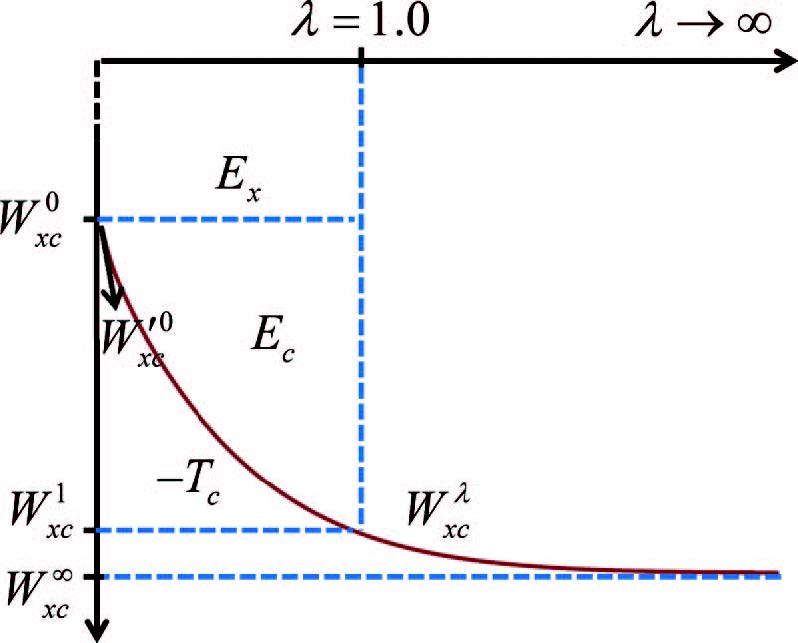
\includegraphics[width=0.5\textwidth]{assets/adiabatic-curve.jpg}
  \caption{绝热路径曲线示意图。下图取自文献\cite{Su-Xu.JCP.2014}。图中的 $W_{xc}^{\lambda}$ 即本文中的 $\mathcal{W}_{\lambda}$。图中的 $W'_{xc}{}^{0}$ 数值上等于 $2 E_\mathrm{GL}^{(2)}$。}
  \label{fig.2.adiabatic-curve}
\end{figure}

为提升测评精度,其中一种有效且理论上相对严格的策略,是结合 G\"orling-Levy 微扰与传统的低阶密度泛函近似,对 $\mathcal{W}_{\lambda}$ 作合理的参数化。尽管传统的低阶 (在“Jacob 阶梯”的第四阶或以下,即杂化泛函或以下的) 泛函未必能正确地描述 $\mathcal{W}_{\lambda}$ 在 $\lambda \rightarrow 0$ 时的行为,但却因为对 $\mathcal{W}_{\lambda}$ 在 $\lambda \in [0, 1]$ 整体有良好的描述,传统泛函的 $E_\mathrm{xc} [\rho]$ 的结果通常相比于 GLPT2 要来地更精确。如果在构造绝热路径曲线 $\mathcal{W}_{\lambda}$ 的过程中,在 $\lambda \rightarrow 0$ 时偏重 G\"orling-Levy 微扰理论、而在 $\lambda \rightarrow 1$ 时偏重传统泛函,那么可以取两者所长,获得比传统泛函近似或 GLPT2 更为精确的泛函。在这种新的泛函形式中,交换相关能同时有严格交换能 $E_\mathrm{x}^\mathrm{exact}$ 与二阶微扰相关能 $E_\mathrm{GL}^{(2)}$ 的掺杂:
\begin{equation}
  E_\mathrm{xc} = \int_0^\lambda \mathcal{W}_{\lambda} \, \mathrm{d} \lambda = E_\mathrm{xc}^\text{low-rung} + c_\mathrm{x} E_\mathrm{x}^\mathrm{exact} + c_\mathrm{c} E_\mathrm{GL}^{(2)}
\end{equation}
因此这类泛函近似成为双杂化泛函。

许多在测评结果上有优异表现的双杂化泛函,譬如 B2PLYP、XYG3 等,通过上述策略对将双杂化泛函近似合理化\cite{Grimme-Grimme.JCP.2006, Zhang-Goddard.PNAS.2009};但在实践中,则是直接对 $E_\mathrm{xc} [\rho]$ 中的参数 $c_\mathrm{x}, c_\mathrm{c}$ 在数据集下作拟合,而没有直接构造 $\mathcal{W}_{\lambda}$ 本身。以 PBE-ACDH\cite{Su-Xu.JCP.2014} 为代表的一类泛函,则是使用参数或模型构造 $\mathcal{W}_{\lambda}$ 并对 $\lambda$ 作积分,得到 $E_\mathrm{xc} [\rho]$。

需要指出,对绝热路径曲线 $\mathcal{W}_{\lambda}$ 作参数化或模型化后积分,从而在 $E_\mathrm{xc}$ 中引入 GLPT2 相关能,是双杂化泛函的其中一种理论基础。以 PBE0-DH\cite{Toulouse-Adamo.JCP.2011} 为代表的双杂化泛函,其理论基础并非构建于 $\lambda = 0$ 的 Kohn-Sham 轨道行列式下 G\"orling-Levy 微扰,而是构建于 $0 < \lambda < 1$ 下杂化泛函轨道行列式下的二阶微扰基础上\cite{Sharkas-Savin.JCP.2011};该理论不需要引入绝热路径。

不论是使用绝热路径、还是使用杂化泛函波函数下的微扰理论,都可以构造出双杂化泛函。但与低阶泛函中纯粹以理论模型驱动所构造 PBE、TPSS、SCAN 或他们对应的杂化泛函在诸多数据集下测评表现,相对于同等级参数拟合方法仍然有不少优势\cite{Goerigk-Grimme.PCCP.2017, Medvedev-Lyssenko.S.2017}的情况不同,存在经验参数的双杂化泛函近似通常要比纯理论模型驱动构造的泛函有更优异的测评表现\cite{Mehta-Goerigk.PCCP.2018}。因此,理论模型通常在双杂化泛函中扮演的角色,很可能是对双杂化泛函的合理化。若要提升双杂化泛函的测评数值表现,参数优化非常重要。

但理论模型仍然可以指导双杂化密度泛函的发展。目前在数值计算上的迹象表明,绝热路径曲线通常是凸曲线\cite{Frydel-Burke.JCP.2000, Fuchs-Burke.JCP.2005, Teale-Helgaker.JCP.2009,Teale-Helgaker.JCP.2010, Carrascal-Burke.JPCM.2015} (但目前没有确切的证明\cite{Crisostomo-Burke.LMP.2023}):
\begin{equation}
  \frac{\mathrm{d}^2}{\mathrm{d} \lambda^2} \mathcal{W}_{\lambda} \geqslant 0, \quad \lambda \in [0, 1] \quad \text{(conjecture)}
\end{equation}
这意味着图 \ref{fig.2.adiabatic-curve} 所示的绝热路径曲线 $\mathcal{W}_\lambda$,数值上必然不小于以 $E_\mathrm{x}^\mathrm{exact}$ 为零点、以 $2 E_\mathrm{GL}^{(2)}$ 为斜率的直线;进而对 $\mathcal{W}_\lambda$ 积分后,存在的关系式是
\begin{equation}
  E_\mathrm{xc} \geqslant E_\mathrm{x}^\mathrm{exact} + E_\mathrm{GL}^{(2)} \quad \text{(conjecture)}
\end{equation}
或者等价地,GLPT2 相关能相对于真实体系相关能必然有一定的负误差:
\begin{equation}
  E_\mathrm{GL}^{(2)} \leqslant E_{\mathrm{c}, \lambda=1} \quad \text{(conjecture)}
\end{equation}
作为具体的例子,在低阶密度泛函近似所给出的能量相对精确、且所给出的 Kohn-Sham 轨道足够精确的前提下,若要在能量计算中引入 GLPT2 相关能,那么对于下述泛函模型
\begin{equation*}
  E_\mathrm{xc}^\mathrm{DH} = c_\mathrm{x} E_\mathrm{x}^\mathrm{exact} + c_\mathrm{x}^\text{low-rung} E_\mathrm{x}^\text{low-rung} + c_\mathrm{c} E_\mathrm{GL}^{(2)} + c_\mathrm{c}^\text{low-rung} E_\mathrm{c, \lambda=1}^\text{low-rung}
\end{equation*}
我们应当预期
\begin{equation*}
  c_\mathrm{c} + c_\mathrm{c}^\text{low-rung} \leqslant 1 \quad \text{(conjecture)}
\end{equation*}
事实上,在 xDH@B3LYP 模型下的诸多泛函的优化结果印证了这个结论\cite{Zhang-Xu.JPCL.2021}。因此,要求 $c_\mathrm{c}, c_\mathrm{c}^\mathrm{low-rung}$ 等相关能参数之和小于 1,是其中一种引入 GLPT2 相关能以构造双杂化泛函的限制条件。

同时,G\"orling-Levy 微扰理论本身是类似于波函数方法、通过微扰阶数增加而逐步逼近真实泛函的理论框架;因为微扰阶数的增加会导致计算资源的巨量消耗,现在的密度泛函近似避免使用更高阶的 G\"orling-Levy 微扰相关能而仅考虑 GLPT2。但注意到波函数理论中存在一些近似方法:它们在 M\o{}ller-Plesset 微扰或耦合簇理论的框架下,基于较低阶的近似,引入一部分计算量较小的高阶贡献。对应于 MP2 的计算消耗,介于 MP2 到 CCSD 的经典波函数方法有 IEPA\cite{Sinanoǧlu-Sinanoǧlu.ACP.1964, Nesbet-Nesbet.ACP.1965}、MP2/cr\cite{Dykstra-Davidson.IJQC.2000}、CC2\cite{Christiansen-Joergensen.CPL.1995} 等。在下一节中,我们将会回顾 IEPA 与 MP2/cr 方法,并表明这类方法的相关能将大于 MP2 的相关能。由于 GLPT2 相关能通常近似为基于 Kohn-Sham 轨道行列式的 MP2 相关能,而 GLPT2 相关能相对于真实体系的相关能 $E_\mathrm{c, \lambda=1}$ 总是负误差;同时,由于 G\"orling-Levy 微扰中包含 $\hat V_\mathrm{ee}$ 算符,因而一部分表达式预期与 M\o{}ller-Plesset 微扰有着同样的结构,在能量计算中引入高阶的基于 Kohn-Sham 轨道行列式的 M\o{}ller-Plesset 微扰能量是合理的;因此,在双杂化泛函近似中引入 IEPA 或 MP2/cr 等相关能,预期一定程度上可以化解 GLPT2 的负误差,并且是理论上合理的。

\section{理论背景:电子对方法}
\label{sec.2.iepa-theory}

若参考态为 Hartree-Fock 基态 $| 0 \rangle$,且依据 Brillouin 定理的推论认为在 Fock 算符下的一次激发态可以近似忽略,那么真实的、含有相关效应的波函数可以写为
\begin{equation}
  | \Psi \rangle = | 0 \rangle + \sum_{ijab} t_{ij}^{ab} | {}_{ij}^{ab} \rangle + \cdots
\end{equation}
上式中,$| {}_{ij}^{ab} \rangle$ 表示 Hartree-Fock 二次激发波函数 $a_a^\dagger a_b^\dagger a_j a_i | 0 \rangle$;$a_i, a_j$ 表示对占据轨道 $i, j$ 的湮灭算符、$a_a^\dagger, a_b^\dagger$ 表示对非占轨道的产生算符。在这里,$t_{ij}^{ab}$ 称为二次激发系数 (对于耦合簇理论,也称为二次簇算符系数)。对于本工作所提及的所有 post-HF 方法,在忽略一次激发态的前提下,相关能总是可以表示为二次激发系数与双电子积分的乘积和:
\begin{equation}
  E_\mathrm{c} = \frac{1}{4} \sum_{ijab} t_{ij}^{ab} \langle ij || ab \rangle
\end{equation}
因此,对二次激发系数 $t_{ij}^{ab}$ 计算方式的差异,区分了不同 post-HF 方法。

在本工作中,我们涉及的电子对方法是 IEPA 及其变种 sIEPA、以及 MP2/cr。大体来说,这些方法可以通过精确的方法一步一步近似得到。依照精度与计算消耗从大到小的排序,
\begin{itemize}[nosep]
  \item \textbf{Full-CI。}该方法将所有基于 Fock 算符下基态下的激发态作为变分空间,对分子体系的 Hamilton 算符 $\hat H$ 求取变分极小。在有限基组下,若不考虑溶剂化、分子振动、精细光谱以及其它实验化学影响下,该方法是最精确的计算化学方法;
  \item \textbf{CCD}\cite{Coester-Coester.NPB.1958, Coester-Kuemmel.NPB.1960, Cizek-Cizek.JCP.1966, Cizek-Paldus.IJQC.1971}\textbf{。}将高次 Hartree-Fock 激发态 (在 Fock 算符下的激发) 近似为二次簇算符的耦合。该方法满足正交不变性 (unitary invariance) 与大小延展性 (size extensivity) 等重要的物理条件,且计算精度相对较高;但需要多次 $O(n_\mathrm{occ}^2 n_\mathrm{vir}^4)$ 复杂度的计算、且内存资源消耗巨大。
  \item \textbf{CEPA}\cite{Ahlrichs-Ahlrichs.CPC.1979}\textbf{。}将 CCD 簇算符系数方程中的部分项近似为零,以对计算过程中复杂度为 $O(n_\mathrm{occ}^2 n_\mathrm{vir}^4)$ 的巨量计算与内存消耗的项作非占轨道的解耦,从而仅耦合占据电子对。该方法以牺牲一定的精度与正交不变性为代价,换取计算效率的改善、并仍然保证大小延展性的性质。由于解耦非占轨道的方式不唯一,CEPA 存在四种不同的近似形式。
  \item \textbf{CPF}\cite{Ahlrichs-Ehrhardt.JCP.1985}\textbf{。}该方法是基于 CID (\underline{C}onfiguration \underline{I}nteraction \underline{D}oubles) 的改善。CPF 方法中,变分所涉及到的分母不同于波函数归一化量 $\langle \Psi | \Psi \rangle$,而是电子对的相关波函数的归一化量。该方法也具有大小延展性,且与 CEPA(1) 方法有所联系。
  \item \textbf{IEPA}\cite{Sinanoǧlu-Sinanoǧlu.ACP.1964, Nesbet-Nesbet.ACP.1965}\textbf{。}以 CEPA(2) 为基础,进一步地解耦成对占据轨道。
  \item \textbf{MP2/cr}\cite{Dykstra-Davidson.IJQC.2000}\textbf{。}以 CPF 方法为基础,忽略部分残差项近似而来。亦可以 CEPA(1) 为基础,通过激进近似给出。
  \item \textbf{MP2}\cite{Moeller-Plesset.PR.1934}\textbf{。}对于所有上述涉及到的方法,在求取激发系数 $t_{ij}^{ab}$ 时忽略所有二阶及以上的微扰项、或在求取相关能时忽略所有三阶及以上的微扰项。
\end{itemize}

简要回顾 IEPA 与 MP2/cr 的具体表达式。对于 IEPA 方法,其能量可以拆解为成对占据电子的贡献总和:
\begin{equation}
  E_\mathrm{c}^\mathrm{IEPA} = \frac{1}{2} \sum_{ij} e_{ij}
\end{equation}
电子对 $ij$ 的相关能则表示为
\begin{equation}
  e_{ij} = \frac{1}{2} \sum_{ab} \frac{|\langle ij || ab \rangle|^2}{D_{ij}^{ab} + e_{ij}} \quad \text{(IEPA)}
\end{equation}
其中,$D_{ij}^{ab}$ 是轨道能差 $\varepsilon_i + \varepsilon_j - \varepsilon_a - \varepsilon_b$。作为参照,MP2 的电子对相关能表示为
\begin{equation}
  e_{ij} = \frac{1}{2} \sum_{ab} \frac{|\langle ij || ab \rangle|^2}{D_{ij}^{ab}} \quad \text{(MP2)}
\end{equation}
从程序实现的角度,IEPA 方法需要迭代、而 MP2 方法则可以一次性地给出电子对能量。对于 HOMO/LUMO gap 较小的体系,若此时的 $i, j$ 代表 HOMO 轨道、$a, b$ 代表 LUMO 轨道,则 $D_{ij}^{ab}$ 的数值较小、但 $e_{ij}$ 会因为作为分母的 $D_{ij}^{ab}$ 较小而有较大的数值。对于 MP2 方法,当 $D_{ij}^{ab}$ 接近零时,$e_{ij}$ 将会接近负无穷大;但对于 IEPA 方法,由于较大数值的 $e_{ij}$ 也在分母中,因而避免了 $e_{ij}$ 趋于负无穷大的趋势。因此,IEPA 方法在 HOMO/LUMO gap 较小的体系,特别是分子解离曲线问题上,相对于 MP2 有更好的表现\cite{Zhang-Scheffler.NJP.2016, Zhang-Scheffler.PRL.2016}。

对于 MP2/cr 方法,它相对于 MP2 方法而言,电子对相关能缩放了一个比例 $N_{ij}$:
\begin{equation}
  e_{ij} = \frac{1}{2} \sum_{ab} \frac{1}{N_{ij}} \frac{|\langle ij || ab \rangle|^2}{D_{ij}^{ab}} \quad \text{(MP2/cr)}
\end{equation}
其中,比例系数定义为
\begin{equation}
  N_{ij} = 1 + \frac{1}{2} \sum_{kab} \big( (t_{ik}^{ab})^2 + (t_{jk}^{ab})^2 \big) \quad \text{(MP2/cr)}
\end{equation}
从程序实现的角度,MP2/cr 与 MP2 方法一样,可以一次性地给出电子对能量。对于 HOMO/LUMO gap 较小的体系,由于置于分母中的比例系数 $N_{ij}$ 中包含较大的激发张量平方 $(t_{ij}^{ab})^2$,因此也可以避免 $e_{ij}$ 过快地区域负无穷大的趋势。该方法同样在分子解离曲线上,相比于 MP2 有更好的表现\cite{Dykstra-Davidson.IJQC.2000}。

由于 IEPA 与 MP2/cr 方法均是增加分母的绝对值;而相关能本身是负值,因此这两个方法一定会给出比 MP2 相关能更大的 (绝对值上更小的) 相关能。回顾到先前关于绝热路径的讨论,可以认为这类方法相对于 MP2 考虑了更多的高阶微扰贡献、且有希望更好地满足绝热路径曲线的凸性。我们预期在密度泛函中引入这类电子对方法的相关能形式,特别在 HOMO/LUMO gap 较小的体系,有望提升泛函的测评精度。

\section{实现细节}

\subsection{数据集与误差量标}

在本工作中,我们将使用 GMTKN55 全数据集\cite{Goerigk-Grimme.PCCP.2017}与 Minnesota 2015 其中五个数据子集\cite{Yu-Truhlar.PCCP.2015} (MR-MGM-BE4、MR-MGN-BE17、MR-TM-BE13、SR-MGM-BE9、SR-TM-BE17),作为泛函表现的量标。这两个数据集的子集说明列于表 \ref{tab.2.subset-detail}。其中,Minnesota 2015 数据子集中的“单参考”与“多参考”,是指在波函数或密度泛函方法计算下,依据一定的指标特征\cite{Lee-Taylor.IJQC.1989, Schultz-Truhlar.JPCA.2005, Zhao-Truhlar.JCTC.2006, Tishchenko-Truhlar.JCTC.2008},若体系的 Hartree-Fock 参考态在考虑相关效应的波函数中占据较大的比例,则称该体系为单参考 (single-reference) 的;否则是多参考 (multi-reference) 的。

\begin{table}[h]
\centering
\caption{测评数据集概况与参数拟合权重。}
\label{tab.2.subset-detail}
\widetabular{
  \begin{tabular}{llllr}
  \toprule
  数据集         & 子集名称\tnote{a}        & 化学问题        & 反应数据数 & 权重 \\
  \midrule
  GMTKN55        & Sub1        & 基本性质与小体系反应能 & 473 & 48\%\tnote{b} \\
                & Sub2        & 大体系反应能与异构能  & 243 &  \\
                & Sub3        & 反应势垒        & 194 &  \\
                & Sub4        & 分子间非共价相互作用  & 291 &  \\
                & Sub5        & 分子内非共价相互作用  & 304 &  \\ \hdashline
  Minnesota 2015 & MR-MGM-BE4  & 多参考主族金属键能   & 4 & 12\% \\
                & MR-MGN-BE17 & 多参考主族非金属键能  & 17 & 8\% \\
                & MR-TM-BE13  & 多参考过渡金属键能   & 13 & 12\%  \\
                & SR-MGM-BE9  & 单参考主族金属键能   & 9  & 8\%  \\
                & SR-TM-BE17  & 单参考过渡金属键能   & 17 & 12\%  \\
  \bottomrule
  \end{tabular}
}{
  \item[a] 对于 GMTKN55 数据集,这里列出的 Sub$n$ ($n = 1, 2, 3, 4, 5$) 是大子集;它囊括其它种类的小子集。在本工作中,我们将很少细致地考察 GMTKN55 的小子集测评情况;因此本工作一般称 GMTKN55 的大子集为子集。
  \item[b] GMTKN55 数据集所有子集的 WTMAD-2 权重。
}
\end{table}

测评 GMTKN55 所使用的误差量标是 WTMAD-2:
\begin{equation}
  \text{WTMAD-2} = \frac{1}{\sum_{i}^{n_\mathrm{sub}} N_i} \cdot \sum_{i}^{n_\mathrm{sub}} N_i \cdot \frac{\SI{56.84}{kcal.mol^{-1}}}{\overline{|\Delta E|}_i} \text{MAD}_i
\end{equation}
其中,上式的 $n_\mathrm{sub}$ 是测评数据集的小子集数量、$N_i$ 是小子集 $i$ 的反应数据数量、$\overline{|\Delta E|}_i$ 是小子集 $i$ 反应能参考值的平均绝对值、$\text{MAD}_i$ 是泛函近似在小子集 $i$ 上误差的平均绝对值。该测评量标使得反应前后能量差较大的情形 (譬如燃烧焓、键能、电离能等问题) 允许较大的能量误差、而能量差较小的情形 (譬如弱相互作用、配位效应、分子异构等问题) 则有更苛刻的精度要求,从而较好地平衡了不同反应类型的误差标准。

测评 Minnesota 2015 数据子集的误差量标是 MUEPB,即计算误差时先除以断键数量再取平均绝对值。因此,MUEPB 并非反应能量的误差量标、而是均摊到每个分子键后的键能误差量标。该量标不区分化学键种类,即对单键、双键、三键、配位键一视同仁。

需要指出的是,GMTKN55 数据集与 Minnesota 2015 数据集存在一定的重合。举例来说,Minnesota 2015 数据集中的 MR-MGN-BE17 (多参考主族非金属键能,测评 \ce{CO}、\ce{O2}、\ce{N2} 等主族小分子键解离能) 子集中部分分子收录到 GMTKN55 子集 Sub1 中的 W4-11 (Weizmann-4 原子化能) 小子集;MR-MGM-BE4 (多参考主族金属键能,测评 \ce{CaO}、\ce{MgS} 等体系的键解离能) 与 SR-MGM-BE9 (单参考主族金属键能,测评 \ce{AlCl3}、\ce{AlF3}、\ce{NaO} 等分子的键解离能) 子集的部分分子同时收录到 GMTKN55 子集 Sub1 中的 W4-11 与 ALKBDE10 (碱金属键解离能) 小子集。由于大多数经过经验参数拟合的泛函,其拟合数据集通常与 GMTKN55 较为接近,因此这类泛函在部分数据集 (特别是 MR-MGN-BE17 与 SR-MGM-BE9) 上的表现通常较好。而相应地,尽管 SR-TM-BE13 的计算体系被认为是单参考的,但绝大多数经验参数拟合的密度泛函近似没有将过渡金属纳入拟合数据中、或没有针对过渡金属问题对泛函表达式进行优化,因此多数泛函的测评结果较差。因此,从这部分的测评结果来看,计算体系是否纳入了近似泛函所使用的拟合数据集、以及这类计算问题是否以更大权重地被近似泛函所拟合,相比于计算问题与近似泛函是否同样有单参考的结构,对近似泛函的计算表现影响更重要。部分当前主流的双杂化泛函在 GMTKN55 数据集与 Minnesota 2015 数据集的测评结果列于表 \ref{tab.2.bench-current-gmtkn55-minnesota}。

\begin{sidewaystable}
\centering
\caption{现有泛函在 GMTKN55 全数据集与 Minnesota 2015 部分子集的测评结果。单位 \si{kcal.mol^{-1}}。}
\label{tab.2.bench-current-gmtkn55-minnesota}
\widetabular{
  \begin{tabular}{ld{1.3}d{1.3}d{2.2}d{2.2}d{2.2}d{2.2}d{2.2}d{2.2}}
  \toprule
  & \multicolumn{2}{c}{GMTKN55} & \multicolumn{5}{c}{Minnesota 2015\tnote{a}} & \\
  \cmidrule(lr){2-3} \cmidrule(lr){4-8}
  Functional      &
  \multicolumn{1}{c}{disp.\tnote{b}} & \multicolumn{1}{c}{no disp.} &
  \multicolumn{1}{c}{MR-MGM-BE4} & \multicolumn{1}{c}{MR-MGN-BE17} & \multicolumn{1}{c}{MR-TM-BE13} & \multicolumn{1}{c}{SR-MGM-BE9} & \multicolumn{1}{c}{SR-TM-BE17} &
  \multicolumn{1}{c}{Weighted Error\tnote{c}} \\
  \midrule
  B2GPPLYP        
  & 3.72\tnote{d} & 6.26\tnote{d} & 5.11       & 2.94        & 5.87       & 1.82       & 9.50       & 4.62     \\
  B2PLYP          
  & 5.10\tnote{d} & 8.70\tnote{d} & 6.77       & 2.35        & 4.69       & 2.29       & 9.29       & 5.31     \\
  DSD-BLYP-D3(BJ)   
  & 3.50\tnote{d} & 5.96\tnote{d} & 6.44       & 2.39        & 8.29       & 1.99       & 11.76      & 5.21     \\
  DSD-PBEP86-D3(BJ) 
  & 2.45\tnote{d} & 4.21\tnote{d} & 5.83       & 2.09        & 7.47       & 2.12       & 11.97      & 4.55     \\
  PBE-QIDH        
  & 4.47\tnote{e} & 5.61\tnote{e} & 3.24       & 5.65        & 7.39       & 3.44       & 12.92      & 5.70     \\
  PBE0-DH         
  & 5.54\tnote{e} & 8.13\tnote{e} & 6.54       & 7.58        & 5.59       & 4.07       & 10.02      & 6.25     \\
  TPSS-QIDH       
  & 4.47\tnote{e} & 6.50\tnote{e} & 3.64       & 9.90        & 7.27       & 3.66       & 12.21      & 6.00     \\
  TPSS0-DH        
  & 5.86\tnote{e} & 9.77\tnote{e} & 8.05       & 14.08       & 6.46       & 4.69       & 9.92       & 7.25     \\
  wB97X-2(TQZ)
  & 3.06\tnote{f} & 2.80\tnote{f} & 4.65       & 2.99        & 6.77       & 1.47       & 10.15      & 4.41     \\
  RS-PBE-P86      
  & -               & -               & 2.77       & 4.20        & 7.44       & 3.30       & 15.91      & -        \\
  XYG3            
  & -               & 3.39\tnote{a} & 16.93      & 1.81        & 10.67      & 1.59       & 5.56       & 5.88     \\
  XYG6            
  & -               & 2.18\tnote{a} & 22.85      & 3.97        & 13.20      & 1.78       & 7.23       & 6.70     \\
  XYG7            
  & -               & 2.01\tnote{a} & 17.81      & 2.63        & 12.12      & 2.55       & 6.75       & 5.78     \\
  xDH-PBE0        
  & -               & -               & 18.02      & 4.54        & 8.82       & 2.16       & 10.29      & -        \\
  \bottomrule
  \end{tabular}
}{
  \item[a] Minnesota 2015 部分子集、以及 GMTKN55 下 xDH@B3LYP 模型下泛函 (包括 XYG3、XYG6、XYG7) 的测评数据取自本工作。除 DSD-BLYP-D3(BJ) 与 DSD-PBEP86-D3(BJ) 外,其余泛函在 Minnesota 2015 集合下的测评没有使用色散矫正。XYG3、XYG6、XYG7 的测评结果与文献\cite{Zhang-Xu.JPCL.2021}有一定差距,这是因为本工作与该文献使用了不同的基组与冻核近似规则。
  \item[b] 色散矫正模型均选用 DFT-D3(BJ)。
  \item[c] 在计算加权误差时,选取 GMTKN55 误差较低的数值 (一般来说,若有色散矫正,则使用矫正后的 WTMAD-2 误差),测评结果。
  \item[d] 数据取自文献\cite{Goerigk-Grimme.PCCP.2017}。
  \item[e] 数据取自文献\cite{Mehta-Goerigk.PCCP.2018}。
  \item[f] 数据取自文献\cite{Santra-Martin.JPCA.2019}。
}
\end{sidewaystable}

在后续的工作中,我们将对上述数据集进行参数拟合,构造新的密度泛函。该拟合过程选用的误差量标是 GMTKN55 数据集的 WTMAD-2 误差、与 Minnesota 2015 五个子数据集的 MUEPB 误差的加权 (Weighted Error)。权重列于表 \ref{tab.2.basis-gmtkn55}。该权重是人为设置的;其设置方式反映的是我们对新泛函所能应用的化学问题范围与能力的期许。
\begin{itemize}[nosep]
  \item 设置 GMTKN55 数据集的权重为 48\%,目的是期望参数拟合后的泛函仍然能在诸多主族化学问题中有良好的表现;
  \item 设置 MR-MGM-BE4、MR-TM-BE13、SR-TM-BE17 数据集的权重为 12\%,目的是期望在不严重破坏诸多主族化学计算问题的表现的同时,针对现有泛函难以计算准确的问题作改善;对于表 \ref{tab.2.bench-current-gmtkn55-minnesota} 中所测评的 xDH@B3LYP 模型泛函,除了单参考、多参考过渡金属键解离问题外,主族碱金属的表现也欠佳,因此对这三类化学体系都加以较大的拟合权重;
  \item 设置 MR-MGN-BE17、SR-MGM-BE9 数据集的权重为 8\%;这两类计算问题下 xDH@B3LYP 模型泛函的测评表现良好;权重数值设置得较小,目的是避免对过渡金属键解离问题过拟合。
\end{itemize}

\subsection{数据集计算细节}

本工作所使用的程序已公开\cite{dh.ajz34},该程序基于 \textsc{PySCF} 2.2.1 实现\cite{Sun-Chan.WCMS.2018, Sun-Chan.JCP.2020}。双杂化能量泛函的计算使用 \textsc{dh} 程序 v0.1.9\footnote{https://gitee.com/ajz34/pyscf-forge/tree/dh-v0.1.9/} 与 commit 80ca9e8\footnote{https://github.com/ajz34/pyscf-forge/commit/80ca9e8c3e86943077e5802b3621118fdef73146}。在正文中出现的计算任务没有使用波函数稳定性分析,所有自旋投影 $S_z$ 为零的体系使用限制性 Kohn-Sham 轨道、而 $S_z$ 非零的体系使用非限制性 Kohn-Sham 轨道进行计算。

GMTKN55 数据集计算选用的基组列于表 \ref{tab.2.basis-gmtkn55}。其中,基组 daug-def2-universal-jkfit 是针对 def2-universal-jkfit 基组,使用基于 Woon 与 Dunning 所提出的方法\cite{Woon-Dunning.JCP.1994},在各角量子数上增加两个弥散基函数;增加弥散基函数所用的程序是 \textsc{Basis Set Exchange} 的 \textsc{Python} API\cite{Feller-Feller.JCC.1996, Schuchardt-Windus.JCIM.2007, Pritchard-Windus.JCIM.2019}。GMTKN55 计算所选用的冻核近似规则列于表 \ref{tab.2.fc-gmtkn55}。Minnesota 2015 数据集所选用的基组是 def2-QZVPP\cite{10.1007/BF01112983, 10.1007/BF00528565, 10.1063/1.1622924, 10.1063/1.1305880, 10.1007/s002149900101, 10.1016/0009-2614(96)00382-x, 10.1063/1.459993, 10.1007/bf01114537, 10.1039/b508541a, 10.1063/1.1406535, 10.1063/1.456066, 10.1021/ct300302u, 10.1063/1.1627293},冻核近似规则为表 \ref{tab.2.fc-gmtkn55} 中的 FC-2 规则。

本工作选用 \textsc{SciPy}\cite{Virtanen-Vazquez-Baeza.NM.2020} 进行泛函参数的优化。优化算法选用 L-BFGS-B 算法\cite{Byrd-Zhu.SJSC.1995},收敛判标是参数梯度模长 (\verb|gtol|) 小于 $10^{-5}$。本工作没有进行严格的全局优化;对于后文表 \ref{tab.2.coeff-xyg6-1-weighted-error} 的参数,优化过程是非对电子能矫正项以 XYG6 的参数、对电子能占比微扰能比例以 0.7 作为初始参数;对于 \ref{sec.2.proportion-iepa-like}、\ref{sec.2.proportion-exchange}、\ref{sec.2.propotion-dataset} 等小节中的参数优化问题与图像绘制过程,则以其对应的原始泛函参数、或图中相邻的数据点作为初始参数优化。

\begin{table}[h]
\centering
\caption{GMTKN55 数据集计算所使用的基组}
\label{tab.2.basis-gmtkn55}
\widetabular{
  \begin{tabular}{lll}
    \toprule
    Basis Type          & Basis                     & Subsets Applied \\
    \midrule
    Conventional        & def2-QZVPPD               & WATER27, RG18, IL16, G21EA, \\
                        &                           & BH76, BH76RC, AHB21, ISOL24  \\
                        & def2-TZVPP                & C60ISO, UPU23 \\
                        & def2-QZVPP                & other 45 subsets of GMTKN55 \\
    \hdashline
    Auxiliary  & daug-def2-universal-jkfit & WATER27, RG18, IL16, G21EA, \\
    (RI-JK)    &                           & BH76, BH76RC, AHB21, ISOL24 \\
                        & def2-universal-jkfit      & other 47 subsets of GMTKN55 \\
    \hdashline
    Auxiliary & def2-QZVPPD-rifit         & WATER27, RG18, IL16, G21EA, \\
    (RI-MP2)  &                           & BH76, BH76RC, AHB21, ISOL24 \\
                        & def2-TZVPP-rifit          & C60ISO, UPU23 \\
                        & def2-QZVPP-rifit          & other 45 subsets of GMTKN55 \\
    \bottomrule
  \end{tabular}
}{}
\end{table}

\begin{table}[h]
\centering
\caption{GMTKN55 数据集计算所使用的冻核近似规则 (Rn 前元素)}
\label{tab.2.fc-gmtkn55}
\widetabular{
  \begin{tabular}{cccccc}
    \toprule
    \multicolumn{2}{c}{FC-0\tnote{a}}  &
    \multicolumn{2}{c}{FC-1\tnote{b}}  &
    \multicolumn{2}{c }{FC-2\tnote{c}}  \\
    \cmidrule(lr){1-2} \cmidrule(lr){3-4} \cmidrule(lr){5-6}
    Core & Elements & Core & Elements & Core & Elements \\
    \midrule
    0              & H--Be    & 0              & H--Be    & 0              & H--B     \\
    2              & B--Mg    & 2              & B--Ar    & 2              & C--Si    \\
    10             & Al--Zn   & 10             & K--Kr    & 10             & P--As    \\
    18             & Ga--Sr   & 18             & Rb--Cd   & 18             & Se--Cd   \\
    28             & Zr--Cd   & 28             & In--Xe   & 28             & Cd--Te   \\
    36             & In--Yb   & 36             & Cs--Yb   & 36             & I--Yb    \\
    46             & Lu--Hg   & 46             & Lu--Hg   & 46             & Lu--Hg   \\
    68             & Tl--Rn   & 60             & Tl--Rn   & 60             & Tl--Rn   \\
    \bottomrule
  \end{tabular}
}{
  \item[a] 该规则取自 ORCA (ver 5.0.2) 默认冻核近似规则\cite{Neese-Neese.WCMS.2012, Neese-Neese.WCMS.2018, Neese-Neese.WCMS.2022},并应用于除下述特例外的所有其它子集。
  \item[b] 该规则应用于 HEAVY28 子集。
  \item[c] 该规则取自文献\cite{Santra-Martin.JPCA.2019}。对金属与过渡金属 (B, Si, Ge, As, Sb, Te),该规则将最靠近价层的电子纳入 post-SCF 的相关能计算;而对于其它非金属,仅有价层电子纳入 post-SCF 的相关能计算。该规则应用于 ALK8、ALKBDE10、HAL59、HEAVYSB11、MB16-43 子集。
}
\end{table}

\subsection{解离曲线计算细节}

分子解离曲线问题的计算中,除作为参考值的 DMC 方法外,其它方法选择 cc-pV5Z 基组\cite{Dunning-Dunning.JCP.1989}。MP2、CCSD、CCSD(T) 方法使用传统四中心二电子积分计算,其它方法使用 RI-JK 与 RI-MP2 算法并使用辅助基组 cc-pV5Z-jkfit\cite{Weigend-Weigend.PCCP.2002} 与 cc-pV5Z-rifit\cite{10.1039/b415208e}。计算程序是 \textsc{PySCF} 与 \textsc{dh} commit 80ca9e8。

对于 DMC 方法,首先选用 ccecp-cc-pVQZ 基组\cite{Bennett-Mitas.JCP.2017} 在 \textsc{PySCF} 下给出 CASSCF 的波函数初猜;随后在 \textsc{PyQMC} 程序\cite{Wheeler-Wagner.JCP.2023}下先进行 1000 组态数量的 15 次 VMC 过程;其次进行 10000 组态数量的 4000 次 DMC,并舍弃前 200 次运行结果作能量计算;最后将时间步长为 0.02、0.01、0.005、0.0025、0.001 Hartree 的 DMC 结果线性外推到 0 时间步长的情形。

本工作的分子解离曲线势能面取用相对能量,且在正文中,所有计算限制使用闭壳层波函数。

\section{结果与讨论}
\label{sec.2.iepa-results}

\subsection{XYG6+1 模型双杂化近似泛函的参数优化}

本工作将基于 xDH@B3LYP 模型\cite{Zhang-Xu.JPCL.2021},进行新泛函的拟合。回顾到 xDH@B3LYP 模型定义为
\begin{align}
  E_\mathrm{xc}^\text{xDH@B3LYP} &= a_1 E_\mathrm{x}^\mathrm{exact} + a_2 E_\mathrm{x}^\mathrm{S} + a_3 E_\mathrm{x}^\mathrm{B88} + a_4 E_\mathrm{c}^\mathrm{VWN3} + a_5 E_\mathrm{c}^\mathrm{LYP} \notag \\
  &\quad + a_6 E_\mathrm{c}^\text{OS-MP2} + a_7 E_\mathrm{c}^\text{SS-MP2}
\end{align}
其中,$E_\mathrm{x}^\mathrm{exact}$ 表示 (Generalized) Kohn-Sham 轨道下的严格交换能,$E_\mathrm{x}^\mathrm{S}$ 表示 LDA 型 Slater 交换能\cite{Bloch-Bloch.ZP.1929,Dirac-Dirac.MPCPS.1930},$E_\mathrm{x}^\mathrm{B88}$ 表示 GGA 型 Becke88 交换能\cite{Becke-Becke.PRA.1988},$E_\mathrm{c}^\mathrm{VWN3}$ 表示 LDA 型 Vosko-Wilk-Nusair 相关能\cite{Vosko-Nusair.CJP.1980} (B3LYP 泛函的构成部分之一\cite{Becke-Becke.JCP.1993,Stephens-Frisch.JPC.1994}),$E_\mathrm{c}^\mathrm{LYP}$ 表示 Lee-Yang-Parr 相关能\cite{Lee-Parr.PRB.1988},$E_\mathrm{c}^\text{OS-MP2}$ 与 $E_\mathrm{c}^\text{SS-MP2}$ 分别代表基于参考态的自旋相反与自旋相同的 MP2 相关能。

xDH@B3LYP 模型总共有 7 个可变参数。XYG7 近似泛函的参数是通过对 GMTKN55 数据集的 WTMAD-2 量标进行优化所得到。而 XYG6 近似泛函的参数则是在下述限制条件下,对 WTMAD-2 量标优化得到:
\begin{equation}
  \label{eq.2.constrain-xyg6}
  a_1 + a_2 + a_3 = 1 \quad \text{(constrain on XYG6)}
\end{equation}

为引入 IEPA-like 相关能,我们引入额外的参数 $a_8$,用以控制 IEPA-like 相关能占总高阶微扰相关能的比例;该模型记为 xDH@B3LYP+1,其形式为
\begin{align}
  E_\mathrm{xc}^\text{xDH@B3LYP+1/cr} &= a_1 E_\mathrm{x}^\mathrm{exact} + a_2 E_\mathrm{x}^\mathrm{S} + a_3 E_\mathrm{x}^\mathrm{B88} + a_4 E_\mathrm{c}^\mathrm{VWN3} + a_5 E_\mathrm{c}^\mathrm{LYP} \notag \\
  &\quad + (1 - a_8) (a_6 E_\mathrm{c}^\text{OS-MP2} + a_7 E_\mathrm{c}^\text{SS-MP2}) \notag\\
  &\quad + a_8 (a_6 E_\mathrm{c}^\text{OS-IEPA-like} + a_7 E_\mathrm{c}^\text{SS-IEPA-like})
\end{align}
上式的 $E_\mathrm{c}^\text{SS-IEPA-like}$ 与 $E_\mathrm{c}^\text{OS-IEPA-like}$ 分别代表基于参考态的自旋相反与自旋相同的 IEPA-like 型的相关能。根据引入到泛函近似的 IEPA-like 种类的不同,它可以代表 MP2/cr ($E_\mathrm{c}^\mathrm{MP2/cr}$)、sIEPA ($E_\mathrm{c}^\mathrm{sIEPA}$) 与 IEPA ($E_\mathrm{c}^\mathrm{IEPA}$) 相关能。MP2 与 IEPA-like 在均是微扰形式的相关能;我们也会用记号 PT 表示总微扰相关效应。

在本工作中,我们将始终对 xDH@B3LYP+1 模型引入 XYG6 的限制 (\ref{eq.2.constrain-xyg6}),并称其为 XYG6+1 模型。对 GMTKN55 全集与 Minnesota 2015 的五个子集进行加权拟合后,XYG6+1/cr、XYG6+1/sIEPA 与 XYG6+1/IEPA 模型的泛函参数如表 (\ref{tab.2.coeff-xyg6-1-weighted-error}) 所示。

对于泛函系数,我们注意到 $E_\mathrm{x}^\mathrm{B88}$ 的比例通常小于零;这一现象也出现在 XYG7 对 GMTKN55 数据集的 WTMAD-2 误差量标参数拟合中。除此之外,代表 $E_\mathrm{c}^\text{IEPA-like}$ 占比的参数 $a_8$ 在 XYG6+1/sIEPA 与 XYG6+1/IEPA 中大于一,意味着在这些泛函中 $E_\mathrm{c}^\text{MP2}$ 的占比小于零;而在 XYG6+1/cr 中参数 $a_8$ 则介于零与一之间。从分子解离问题的表现来看,MP2/cr 对 MP2 的矫正相比于 sIEPA 或 IEPA 通常更为激进;因此 $E_\mathrm{c}^\text{MP2/cr}$ 相关能在 XYG6+1/cr 的占比系数更有可能小于 $E_\mathrm{c}^\text{sIEPA}$ 相关能在 XYG6+1/sIEPA 的占比系数。

\begin{table}[h]
\centering
\caption{XYG6+1 模型泛函在 GMTKN55 全集与 Minnesota 2015 五个子集下参数优化结果。}
\label{tab.2.coeff-xyg6-1-weighted-error}
\widetabular{
  \begin{tabular}{lrd{3.8}d{3.8}d{3.8}}
  \toprule
  参数             & 参数意义 & \multicolumn{1}{c}{XYG6+1/cr} & \multicolumn{1}{c}{XYG6+1/sIEPA} & \multicolumn{1}{c}{XYG6+1/IEPA} \\
  \midrule
  $a_1$ 或 $c_\mathrm{x}$ & $E_\mathrm{x}^\mathrm{exact}$ 系数   &  0.851546   &  0.872368     &  0.716712    \\
  $a_2$\tnote{a}          & $E_\mathrm{x}^\mathrm{S}$ 系数       & [0.209516]  & [0.297015]    & [0.272940]   \\
  $a_3$                   & $E_\mathrm{x}^\mathrm{B88}$ 系数     & -0.061062   & -0.169383     &  0.010348    \\
  $a_4$                   & $E_\mathrm{c}^\mathrm{VWN3}$ 系数    &  0.168713   &  0.334350     &  0.359041    \\
  $a_5$                   & $E_\mathrm{c}^\mathrm{LYP}$ 系数     &  0.204008   &  0.088983     &  0.247560    \\
  $a_6$                   & $E_\mathrm{c}^\text{OS-PT}$ 系数     &  0.460703   &  0.479659     &  0.286591    \\
  $a_7$                   & $E_\mathrm{c}^\text{SS-PT}$ 系数     &  0.214325   & -0.004645     &  0.102393    \\
  $a_8$                   & $E_\mathrm{c}^\text{IEPA-like}$ 占比 &  0.596938   &  1.421052     &  1.108974    \\
  $E_\mathrm{c}^\text{IEPA-like}$ & IEPA 类型 & \multicolumn{1}{c}{$E_\mathrm{c}^\text{MP2/cr}$} & \multicolumn{1}{c}{$E_\mathrm{c}^\text{sIEPA}$} & \multicolumn{1}{c}{$E_\mathrm{c}^\text{IEPA}$} \\
  \bottomrule
  \end{tabular}
}{
  \item[a] 该系数并非参数优化得到,而是通过式 (\ref{eq.2.constrain-xyg6}) 的限制,给出的 $a_2 = 1 - a_1 - a_3$ 的结果。
}
\end{table}

\subsection{XYG6+1 模型泛函测评表现}
\label{sec.2.xyg6-1-model-benchmark}

\begin{table}[h]
\centering
\caption{部分 xDH@B3LYP 模型与 XYG6+1 模型近似泛函在数据集下的测评表现。误差单位 \si{kcal.mol^{-1}}。}
\label{tab.2.bench-xyg6-1}
\widetabular{
  \begin{tabular}{ld{2.2}d{2.2}d{2.2}d{2.2}d{2.2}d{2.2}d{2.2}}
  \toprule
  & \multicolumn{4}{c}{xDH@B3LYP} & \multicolumn{3}{c}{XYG6+1\tabnote{a}} \\
  \cmidrule(lr){2-5} \cmidrule(lr){6-8}
  Datasest & 
  \multicolumn{1}{c}{XYG3} & \multicolumn{1}{c}{revXYG3} & \multicolumn{1}{c}{XYG6} & \multicolumn{1}{c}{XYG7} &
  \multicolumn{1}{c}{MP2/cr} & \multicolumn{1}{c}{sIEPA} & \multicolumn{1}{c}{IEPA} \\
  \midrule
  \textbf{GMTKN55} &&&&&&& \\
  Sub1        & 1.74  & 1.57  & 1.50  & 1.29  & 1.53      & 1.69         & 2.10        \\
  Sub2        & 4.70  & 2.83  & 2.45  & 2.38  & 2.54      & 3.97         & 4.53        \\
  Sub3        & 1.71  & 2.25  & 2.11  & 1.82  & 2.22      & 3.28         & 2.57        \\
  Sub4        & 5.15  & 2.94  & 2.83  & 2.86  & 3.38      & 3.70         & 6.97        \\
  Sub5        & 4.25  & 2.80  & 2.43  & 2.10  & 2.59      & 3.11         & 6.60        \\
  All         & 3.39  & 2.38  & 2.18  & 2.01  & 2.36      & 2.94         & 4.41        \\ \hdashline
  \textbf{Minnesota 2015} &&&&&&& \\
  MR-MGM-BE4  & 16.93 & 21.73 & 22.85 & 17.81 & 3.24      & 3.62         & 2.62        \\
  MR-MGN-BE17 & 1.81  & 3.27  & 3.97  & 2.63  & 1.65      & 2.42         & 3.97        \\
  MR-TM-BE13  & 10.67 & 13.88 & 13.20 & 12.12 & 7.40      & 7.75         & 5.30        \\
  SR-MGM-BE9  & 1.59  & 1.82  & 1.78  & 2.55  & 1.97      & 1.87         & 2.03        \\
  SR-TM-BE17  & 5.56  & 7.37  & 7.23  & 6.75  & 4.86      & 5.61         & 4.59        \\ \hdashline
  Weighted Error & 5.88  & 6.71  & 6.70  & 5.78  & 3.28      & 3.79         & 4.10        \\
  \bottomrule
  \end{tabular}
}{
  \item[a] 为方便排版,表头第二行指代的是 XYG6+1 模型泛函所使用的 IEPA 型相关能 $E_\mathrm{c}^\text{IEPA-like}$ 的具体类型;即 MP2/cr 指代 XYG6+1/cr、sIEPA 指代 XYG6+1/sIEPA、IEPA 指代 XYG6+1/IEPA。
}
\end{table}

首先考察经过参数优化后的诸 XYG6+1 模型在各测评集下的表现。从表 \ref{tab.2.bench-xyg6-1} 中可以看出,在引入 IEPA 型相关能、并对加权误差进行参数化拟合后,XYG6+1 的误差表现总体表现有一定提升。

从 GMTKN55 的测评结果来看,XYG6、XYG7 泛函是直接针对 GMTKN55 的 WTMAD-2 量标进行优化,因此这两个泛函在 GMTKN55 的总体测评结果非常优异、误差小于 2.2 \si{kcal.mol^{-1}}。由于 XYG6+1 模型的优化在 GMTKN55 上的权重为 48\% 而非完全针对 GMTKN55 优化、参数量上 XYG6+1 模型与 XYG7 同样为 7 个参数,因此 XYG6+1 在 GMTKN55 上的误差表现逊于 XYG7 是符合预期的。但即使如此,XYG6+1/cr 与 XYG6+1/sIEPA 的 GMTKN55 测评表现仍然表现良好。其中,XYG6+1/sIEPA 的 WTMAD-2 误差 2.94 \si{kcal.mol^{-1}} 小于 XYG3 的误差 3.39 \si{kcal.mol^{-1}};XYG6+1/cr 的误差 2.36 \si{kcal.mol^{-1}} 小于专门针对 GMTKN55 进行优化的 revXYG3 的误差 2.38 \si{kcal.mol^{-1}}。造成 XYG6+1 模型在 GMTKN55 数据集上 WTMAD-2 误差量标增加的主要化学体系是 Sub4 (分子间非共价相互作用) 与 Sub5 (分子内非共价相互作用)。

对于 Minnesota 2015 部分数据子集的测评结果,所有未引入 IEPA-like 型相关能的方法在 MR-MGM-BE4、MR-TM-BE13 子集上有大于 10 \si{kcal.mol^{-1}} 的 MUEPB 误差;而这一巨大的误差随着 IEPA-like 相关能的引入、以及对这部分数据集进行参数优化,得以降低到 MR-MGM-BE4 子集 4 \si{kcal.mol^{-1}}、MR-TM-BE13 子集 8 \si{kcal.mol^{-1}} 以下。但需要指出的是,在这些 Minnesota 2015 子集的测评结果中,XYG6+1 模型泛函并非在主流杂化或双杂化泛函中表现最佳。举例而言,B2PLYP 与 PBE0-DH 泛函在 MR-TM-BE13 子集的 MUEPB 为 4.69 \si{kcal.mol^{-1}} 与 5.59 \si{kcal.mol^{-1}},相比于 XYG6+1/cr 与 XYG6+1/sIEPA 大约 7.5 \si{kcal.mol^{-1}} 的误差要小许多;但 XYG6+1/cr 与 XYG6+1/sIEPA 泛函在 GMTKN55、MR-MGM-BE4、SR-TM-BE17 等数据集或子集上的有相对更好的表现。因此,XYG6+1 模型泛函尽管并非专精于其中一种化学问题,但在各种问题的表现上达到较好的平衡。

从总体的数值表现来看,XYG6+1/cr 泛函的加权误差 3.28 \si{kcal.mol^{-1}} 是诸多双杂化泛函中最小;且除了 MR-TM-BE13 子集的 MUEPB 误差稍大外,在 GMTKN55 数据集与其它经测评的 Minnesota 2015 数据集上的误差都有非常良好的表现。对于 MR-TM-BE13 子集,相对于 XYG$n$ ($n=3,6,7$),XYG6+1/cr 成功地矫正到一般双杂化泛函的误差水平。因此,我们认为 XYG6+1/cr 在处理主族化学与含金属的分子体系解离能等各类问题上有优异的表现。其它 XYG6+1 模型下的泛函,XYG6+1/sIEPA 与 XYG6+1/IEPA,也有相对良好的结果。

\subsection{参数优化讨论:IEPA-like 相关能占比}
\label{sec.2.proportion-iepa-like}

构造新的 XYG6+1 型泛函时,相对于没有引入 IEPA-like 相关能的 xDH@B3LYP 模型,有三个重要的变化:
\begin{enumerate}[nosep]
  \item 引入 IEPA-like 相关能;
  \item 引入 Minnesota 2015 数据子集;
  \item 重新参数优化。
\end{enumerate}
针对这三个问题对泛函优化结果的影响,我们将这三小节分别进行讨论。下文将考察特定模型下泛函参数变化情况;类如 XYG6+1/cr、XYG7 等上面作为具体泛函名称的术语,在下文中一般将作为参数模型出现。

\begin{figure}[h]
  \centering
  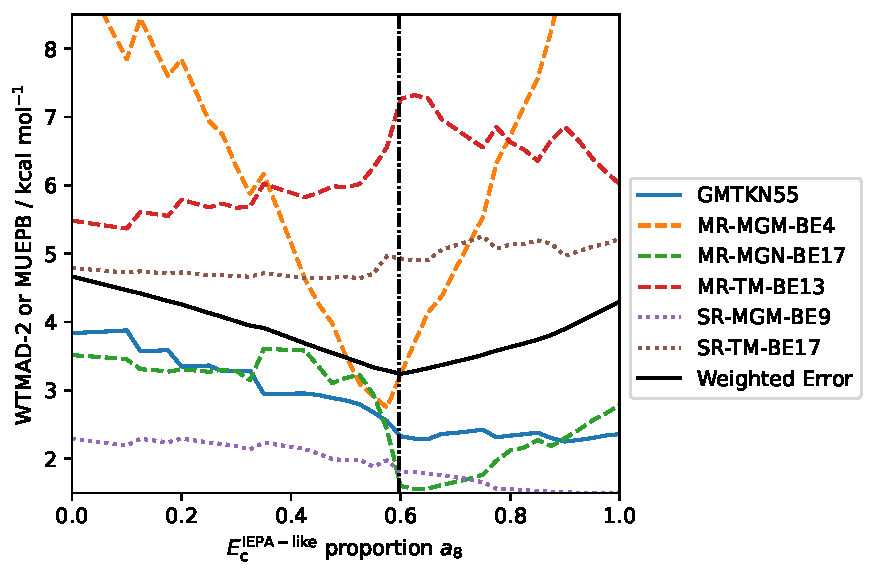
\includegraphics[width=0.6\textwidth]{assets/plot-seq-cr-proportion.pdf}
  \caption{XYG6+1/cr 在限制参数 $a_8$ 下对加权误差的拟合后数据集误差表现。}
  \label{fig.2.plot-seq-cr-proportion}
\end{figure}

首先考虑 IEPA-like 相关能的引入。这里以 XYG6+1/cr 模型为例。图 \ref{fig.2.plot-seq-cr-proportion} 展示的是限制 $E_\mathrm{c}^\text{MP2/cr}$ 在 $E_\mathrm{c}^\mathrm{PT}$ 效应中的占比数 $a_8$ 时,各数据子集误差随 $a_8$ 取值的变化情况。特别地,当取 $a_8 = 0$ (图像最右侧) 时,该模型化归为 XYG6 模型;当取 $a_8 = 1$ (图像最左侧) 时,该模型的微扰相关能完全是 MP2/cr;点划线表示加权误差取到最小时参数 $a_8$ 的数值,即 \ref{sec.2.xyg6-1-model-benchmark} 小节中所定义的 XYG6+1/cr 近似泛函。

受参数 $a_8$ 影响最大的数据集是 MR-MGM-BE4 (多参考主族金属键解离能);若不引入 ($a_8 = 0$) 或完全引入 ($a_8 = 1$) $E_\mathrm{c}^\mathrm{MP2/cr}$ 相关能,其 MUEPB 误差都将超过 8 \si{kcal.mol^{-1}}。事实上,从附录的表 \ref{tab.2.supp.MR-MGM-BE4} 中可以看到,XYG$n$ ($n=3,6,7$) 在 MR-MGM-BE4 测评中,阴离子 \ce{KO-} 与 \ce{LiO-} 的误差很大;其误差分别在 40 \si{kcal.mol^{-1}} 与 20 \si{kcal.mol^{-1}} 左右。这两个体系具有 1 eV 的小 HOMO/LUMO gap,因此可以预期到仅使用 MP2 相关能的 XYG$n$ ($n=3,6,7$) 在这类体系上表现较差。当 $a_8 \simeq 0.6$ 时,MP2/cr 的引入有效地缓解了这两个离子的误差到小于 10 \si{kcal.mol^{-1}},从而 MR-MGM-BE4 子集的 MUEPB 整体误差降至 3 \si{kcal.mol^{-1}} 左右。

对于其它数据集,一般来说,参数 $a_8$ 越大,越有利于 GMTKN55 数据集与 SR-MGM-BE9 子集的误差下降,尽管下降幅度较小;$a_8$ 对于 SR-TM-BE17 数据集的影响不大。需要指出的是,对于 $a_8 \simeq 0.6$ 的情形 (如表 \ref{tab.2.supp.SR-TM-BE17} 所示),SR-TM-BE17 数据集的 \ce{Zr2} 体系 HOMO/LUMO gap 是较小的 1.34 eV,处于 IEPA-like 相关能可以对 MP2 相关能产生有效矫正的范围;在引入 IEPA-like 相关能后计算误差相对于 XYG$n$ ($n=3,6,7$) 下降约 20 \si{kcal.mol^{-1}}。但同时因为其它计算体系的误差有小幅上升,因此 SR-MGM-BE9 子集的整体误差没有下降太多。

值得注意的是 MR-TM-BE13 与 MR-MGN-BE17 的表现在 XYG6+1/cr 模型下 $a_8 = 0.6$ 附近有较大的跳变;这个跳变的影响因素比较可能是间接地因参数优化过程中 $c_\mathrm{x} = a_1$ 即严格交换能的占比跳变较大有关,如图 \ref{fig.2.plot-seq-cr-against-cx} 所示。可以发现,MR-TM-BE13 数据集的 MUEPB 误差通常随严格交换系数 $c_\mathrm{x}$ 的增大而增大;相反地,MR-MGN-BE17 的 MUEPB 误差则随 $c_\mathrm{x}$ 的增大而减小。因此,该误差跳变不能简单地归因于 MP2/cr 的引入本身。关于严格交换能占比参数 $c_\mathrm{x}$ 对各数据集的影响,将在后一小节 \ref{sec.2.proportion-exchange} 中阐述。

\begin{figure}[h]
  \centering
  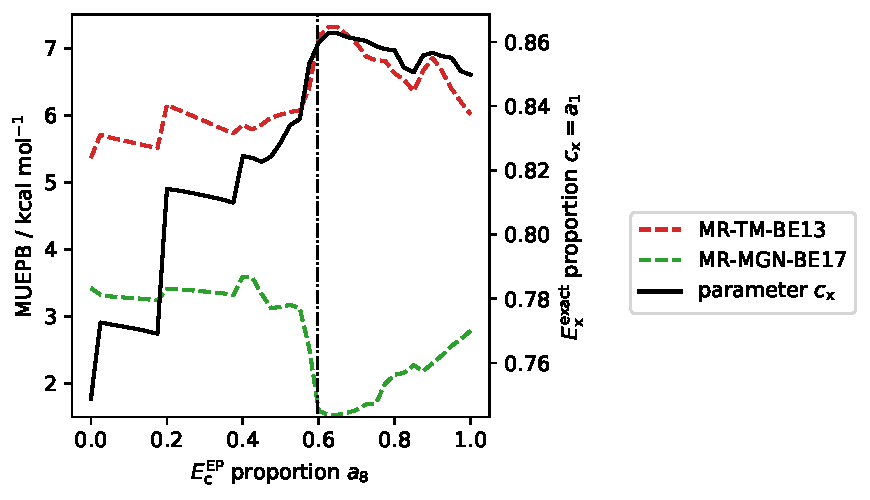
\includegraphics[width=0.6\textwidth]{assets/plot-seq-cr-against-cx.pdf}
  \caption{XYG6+1/cr 在限制参数 $a_8$ 下对加权误差的拟合后 MR-TM-BE13、MR-MGN-BE17 数据集的 MUEPB 误差表现、以及参数 $c_\mathrm{x} = a_1$ 在给定参数 $a_8$ 下的变化情况。}
  \label{fig.2.plot-seq-cr-against-cx}
\end{figure}

在这一小节的最后,我们考察引入 IEPA-like 相关能后表现较差的体系。以 XYG6+1/cr 近似泛函为例,MR-TM-BE13 子集 (表 \ref{tab.2.supp.MR-TM-BE13}) 中的 \ce{TiCl}、\ce{NiCH2+}、\ce{VO} 以及 SR-TM-BE17 子集 (表 \ref{tab.2.supp.SR-TM-BE17}) 中的 \ce{CoH}、\ce{FeH}、\ce{FeCl},这些体系平均每个键的解离误差大于 10 \si{kcal.mol^{-1}}。由于这些体系的 HOMO/LUMO gap 均大于 1.5 eV,因此 MP2/cr 相关能与 MP2 相关能表现上会比较接近,从而难以通过仅引入 MP2/cr 相关能解决这类体系的计算误差。

\subsection{参数优化讨论:严格交换能占比}
\label{sec.2.proportion-exchange}

其次考察严格交换能的占比对数据集测评的影响。图 \ref{fig.2.plot-seq} 展示的是限制严格相关能 $E_\mathrm{x}^\text{exact}$ 在总交换能中的占比数 $c_\mathrm{x} = a_1$ 时,各数据子集误差随 $c_\mathrm{x}$ 取值的变化情况。

首先,从上一小节 \ref{sec.2.proportion-iepa-like} 的讨论中,我们已经注意到 IEPA-like 相关能的引入对 MR-MGM-BE4 子集的 MUEPB 测评表现、特别是 \ce{KO-} 与 \ce{LiO-} 离子的解离能有很大的提升;在图 \ref{fig.2.plot-seq} 中,可以清晰地看到在 $c_\mathrm{x} > 0.5$ 时,XYG6+1 参数模型在 MR-MGM-BE4 的测评结果上明显优于没有引入 IEPA-like 相关能的 XYG$n$ ($n=6,7$)。同时,对于 XYG6+1/cr 模型,其 GMTKN55、MR-MGN-BE17 与 MR-TM-BE13 在 $c_\mathrm{x} > 0.5$ 时的误差相较于 XYG$n$ ($n=6,7$) 有一定提升,SR-MGM-BE9 与 SR-TM-BE17 的误差与 XYG$n$ ($n=6,7$) 接近;考虑到一般的双杂化泛函近似都选用 $c_\mathrm{x} > 0.5$,因此图 \ref{fig.2.plot-seq} 的结果进一步验证了引入 IEPA-like、特别是 MP2/cr 相关能,对整体误差表现确实有所提升。

但对于其它数据集而言,不论选取哪一种模型,总体上
\begin{itemize}[nosep]
  \item $c_\mathrm{x}$ 愈接近 0.9,GMTKN55 数据集的 WTMAD-2 误差愈小;
  \item $c_\mathrm{x}$ 愈接近 0.5,MR-TM-BE13 子集的 MUEPB 误差愈小;
  \item SR-TM-BE17 子集的误差比较平稳,在 $c_\mathrm{x}$ 取 0.7 时通常较小。
\end{itemize}
考虑到 GMTKN55 数据集在拟合过程中的权重较大、MR-TM-BE13 与 MR-MGM-BE4 子集的误差本身较大,且这三个数据集误差对 $c_\mathrm{x}$ 的变化比较敏感,因此对泛函模型进行参数优化时,$c_\mathrm{x}$ 取值事实上平衡这三个数据集的误差。由于 IEPA-like 相关能的引入大幅降低了 MR-MGM-BE4 的误差、并一定程度地降低了 MR-TM-BE13 的误差以及其对 $c_\mathrm{x}$ 取值的敏感程度,因此 XYG6+1 模型所优化得到的参数中 $c_\mathrm{x}$ 取值比较接近 GMTKN55 数据集下表现良好的范围即 $c_\mathrm{x} \simeq 0.9$。而对于 XYG$n$ ($n=6,7$) 模型而言,降低参数 $c_\mathrm{x}$ 可以在牺牲一定的 GMTKN55 误差时显著降低 MR-TM-BE13 与 MR-MGM-BE4 的误差,因此参数这类模型倾向于优化 $c_\mathrm{x}$ 到大约 0.7 左右。

\begin{figure}[h]
  \centering
  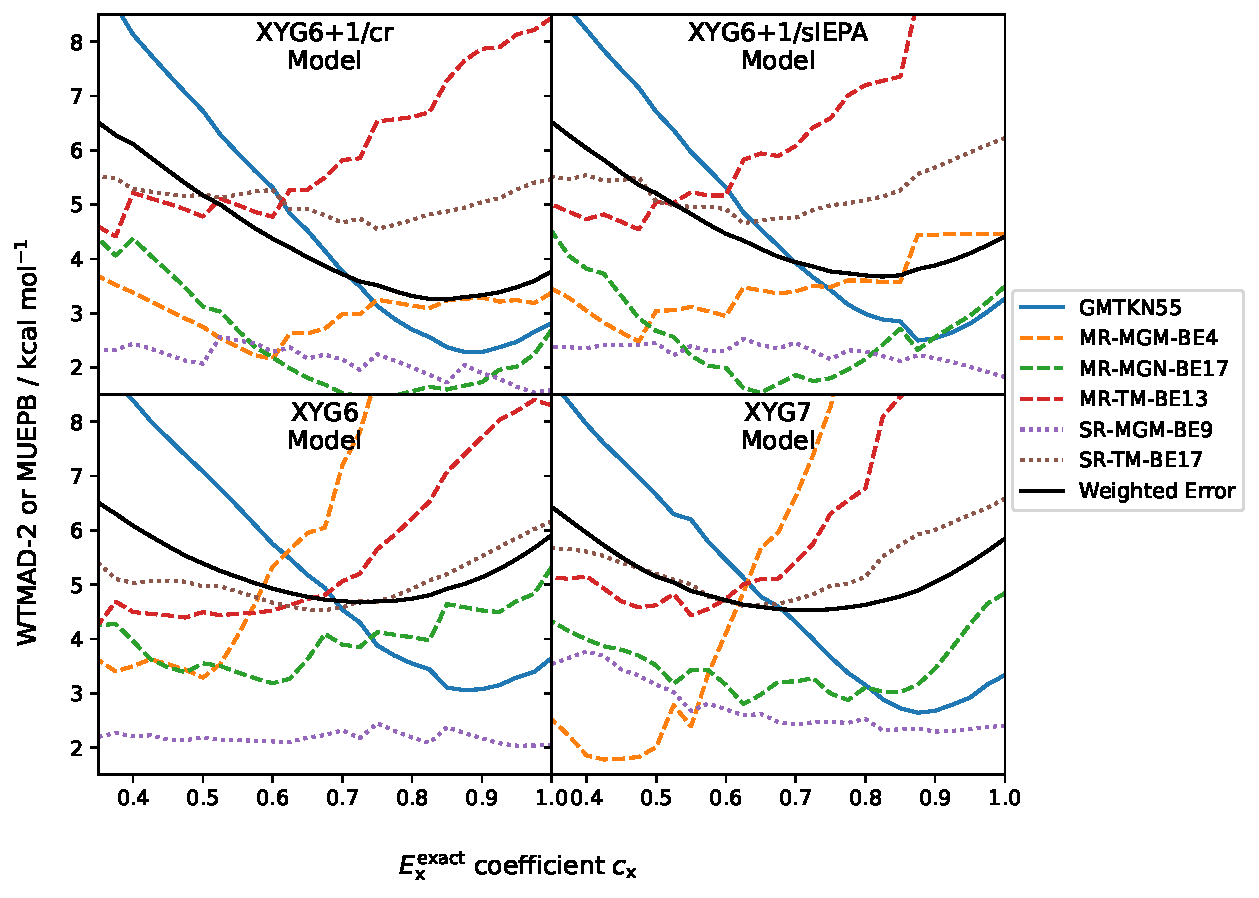
\includegraphics[width=0.9\textwidth]{assets/plot-seq.pdf}
  \caption{诸参数模型在限制参数 $c_\mathrm{x} = a_1$ 下对加权误差的拟合后数据集的误差表现。}
  \label{fig.2.plot-seq}
\end{figure}

Yu 等\cite{Yu-Truhlar.CS.2016} 认为,Hartree-Fock 交换能通常可以提升碳水化合物、弱相互作用、反应能垒等问题上有较好的表现 (这些也是 GMTKN55 数据集着重关心的问题),但会破坏多参考体系问题的表现。尽管 Yu 等的主张是针对杂化泛函所提,但图 \ref{fig.2.plot-seq} 表明在 $c_\mathrm{x} > 0.5$ 的情形下表明基于 B3LYP 轨道的双杂化泛函也有相同的结论。

XYG6+1 模型尽管可以更好地处理以 \ce{KO-}、\ce{LiO-}、\ce{Zr2} 为代表的 HOMO/LUMO gap 较小的计算问题,但需要指出的是,尽管引入了 IEPA-like 型相关能的 XYG6+1 模型一定程度上减少了 MR-TM-BE13 的误差,但减小幅度远小于降低 $c_\mathrm{x}$ 所带来的收益;类如 \ce{TiCl}、\ce{NiCH2+}、\ce{VO}、\ce{CoH}、\ce{FeH}、\ce{FeCl} 等困难的计算问题,一定程度地降低 $c_\mathrm{x}$ 尽管能有更好的计算表现,但同时会推高 GMTKN55 为代表的主族化学问题的误差。因此需要承认,为要更好地解决这两类问题,仅使用引入 IEPA-like 相关能的 XYG6+1 框架仍然是不够的。

\subsection{参数优化讨论:数据集的影响}
\label{sec.2.propotion-dataset}

简单讨论引入 Minnesota 2015 数据集与否,对参数优化结果的影响。图 \ref{fig.2.plot-seq-xyg7} 展示了 XYG6+1/cr 模型下,仅对 GMTKN55 数据集参数优化、与额外引入 Minnesota 2015 五个数据子集参数优化的误差比较。可以看到,引入额外的数据集、并重新定义误差量标,确实会使得部分数据子集的误差表现有明显的变化。引入 Minnesota 2015 数据集进行优化后,在所有图中展示的 $c_\mathrm{x}$ 区域内对 GMTKN55 的 WTMAD-2 误差量标有大约 0.5 \si{kcal.mol^{-1}} 的增加。因此,GMTKN55 的误差总体变化不大;由于我们在构造加权误差时对 GMTKN55 的 WTMAD-2 施加权重为很大的 48\%,因此 GMTKN55 的误差变化较小是可以预期的。

当 Minnesota 2015 五个数据子集纳入拟合集时,尽管每个子集分到的权重不超过 12\%,但除 SR-MGM-BE9 外的数据子集误差显著下降;SR-MGM-BE9 的误差在 $c_\mathrm{x} > 0.5$ 的范围内也可以控制在 3 \si{kcal.mol^{-1}} 以内。这意味着,从积极的角度来看,即使参数拟合没有严重地偏向于每一个参与加权误差计算的 Minnesota 2015 数据子集,XYG6+1/cr 模型也能在不严重影响 GMTKN55 误差的前提下,较好地改善这些子集的表现,从而在更广泛的化学问题上有优异的表现。但从消极的角度看,也意味着在当前的加权误差标准下,这些 Minnesota 2015 子集的误差对 XYG6+1/cr 模型的参数并不是非常稳健;若对加权误差的表达式作较大程度的改变、或引入其它数据集参与参数拟合,这些子集的误差有很大可能会被较大程度地改变。

同时需要注意到,若没有引入 Minnesota 2015 数据子集、而仅以 GMTKN55 数据集进行拟合时,XYG6+1/cr 模型对这五个数据子集 (如图 \ref{fig.2.plot-seq-xyg7} 左侧所示) 的预测表现不能称为良好。若以此现象外推,则不能期望 \ref{sec.2.xyg6-1-model-benchmark} 小节所提出的 XYG6+1/cr 近似泛函可以以与 GMTKN55 和 Minnesota 2015 五个数据子集相同的精度解决被拟合的数据集以外的化学问题。这部分的讨论对除 MP2/cr 以外的其它掺杂 IEPA-like 相关能的 XYG6+1 参数模型泛函同样适用。

\begin{figure}[h]
  \centering
  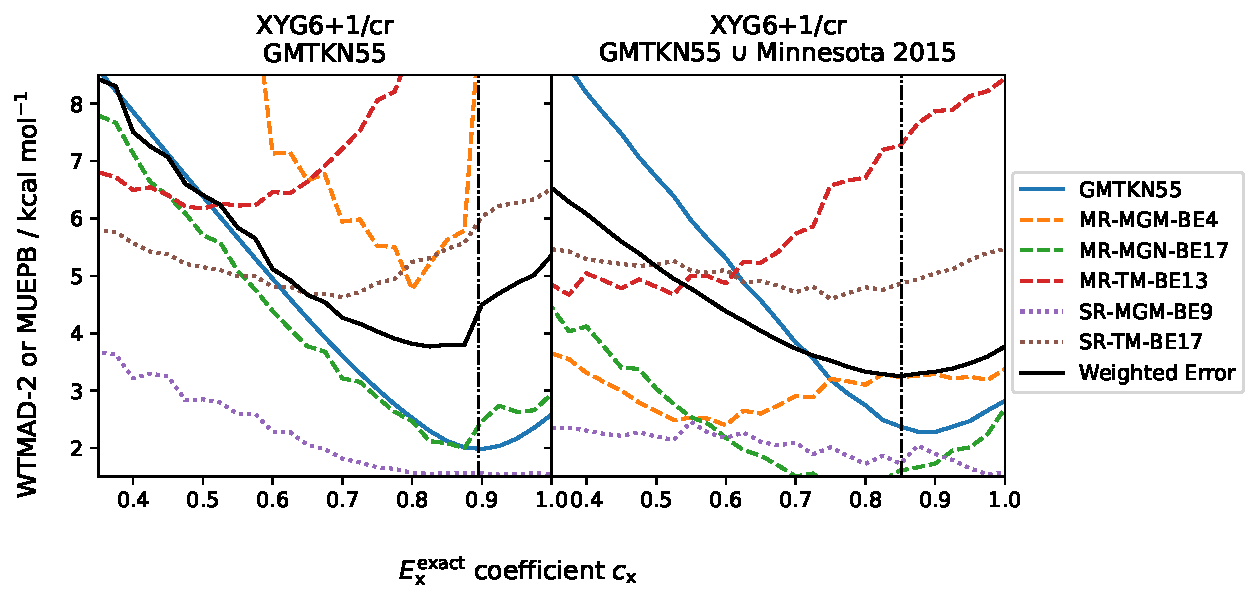
\includegraphics[width=0.9\textwidth]{assets/plot-seq-cr.pdf}
  \caption{XYG6+1/cr 模型在限制参数 $c_\mathrm{x} = a_1$ 下对数据集拟合后数据集的误差表现。\\左图针对 GMTKN55 的 WTMAD-2 误差量标优化,右图针对 GMTKN55 与 Minnesota 2015 五个子集的加权误差量标优化。点划线表示在对应误差量标下 $c_\mathrm{x}$ 的最佳取值。}
  \label{fig.2.plot-seq-xyg7}
\end{figure}

\subsection{XYG6+1 模型泛函在分子解离曲线问题的表现}

在本节最后,将简短地考察 XYG6+1 模型泛函的在部分分子解离曲线问题的表现。

作为三键体系,\ce{N2} 氮气解离问题是最有挑战性的分子解离势能面问题之一。在图 \ref{fig.2.curve-N2} 中可以看到,在解离曲线 1.0--2.0 \AA 的范围内,XYG6+1/cr 方法与 DMC 方法之间的误差普遍在 30 \si{kcal.mol^{-1}} 以内;而 XYG6+1/IEPA 方法与 CCSD(T)、DMC 方法的结果在 1.0--2.0 \AA 非常接近。XYG6+1/sIEPA 尽管存在较大误差,但相较于 MP2、MP2/cr-III、XYG$n$ ($n=3,7$) 等方法,在键长超过 1.4 \AA 时严重下行的趋势上有所改善。

但需要指出,在图中所测评的基于单参考态的近似方法中,几乎没有可以正确预言超过 2.0 \AA 后解离的趋势。CCSD 方法尽管在解离后段趋于准确值 (两个氮原子的能量和),但由于在 1.0--2.0 \AA 区间高估了解离趋势,因此产生了非物理的凸包。CCSD(T) 与 XYG6+1/cr 方法尽管在 1.0--2.0 \AA 的范围内表现良好,但在 2.0 \AA 以后的区域有明显下行趋势。XYG6+1/sIEPA 与 XYG6+1/IEPA 方法则在 2.0 \AA 以后的区域有明显的上行趋势;这是因为尽管 sIEPA 与 IEPA 相关能的趋势是下行,但 MP2 相关能相比于 sIEPA 与 IEPA 相关能下行趋势要明显地多;而 XYG6+1/sIEPA 与 XYG6+1/IEPA 的 MP2 在总微扰型相关能中的占比分别约为 -0.42\% 和 -0.11\%,由于 MP2 相关能负系数的原因,XYG6+1/sIEPA 与 XYG6+1/IEPA 显现出了与 MP2 相反的上升趋势。由于 XYG6+1/sIEPA 中 MP2 相关能的负系数占比更大,因此 XYG6+1/sIEPA 比 XYG6+1/IEPA 更早、更明显地在势能面上显现出错误的上升趋势。

\begin{figure}[h]
  \centering
  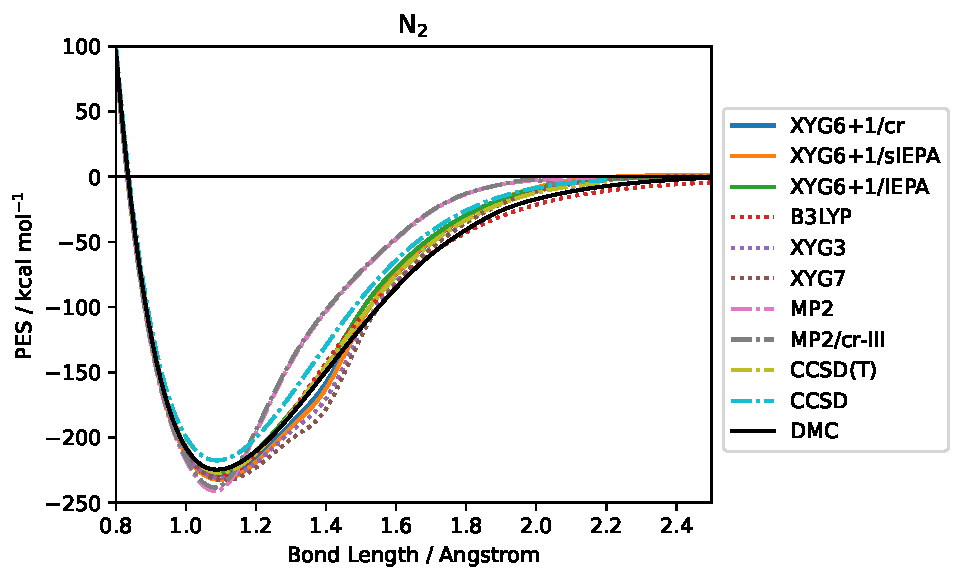
\includegraphics[width=0.7\textwidth]{assets/curve-N2.pdf}
  \caption{各方法在 \ce{N2} 解离曲线的表现。}
  \label{fig.2.curve-N2}
\end{figure}

随后考虑 \ce{F2} 解离曲线。在图 \ref{fig.2.curve-F2} 中,仍然没有方法能完全正确地预言合理的解离趋势。尽管 CCSD(T) 的 \ce{F2} 解离曲线在 1.2 \AA 后始终是倾向于成键的 (势能面的能量在 0 \si{kcal.mol^{-1}} 以下),但在 2.2 \AA 以后显现出不正确的下行趋势。XYG6+1/cr、XYG6+1/sIEPA 与 XYG$n$ (n=3,7) 在 1.2--1.6 \AA 的成键区域中,能量与 CCSD(T) 非常接近。但在 2.0 \AA 后的区域中,XYG$n$ ($n=3,7$) 有着比 CCSD(T) 更加严重的下行。相反地,诸 XYG6+1 近似泛函与 CCSD、B3LYP、MP2/cr-III 等方法则在成键区域以后严重高估势能面;这些方法在 1.6--2.0 \AA 的区域中有比较接近的数值。

\begin{figure}[h]
  \centering
  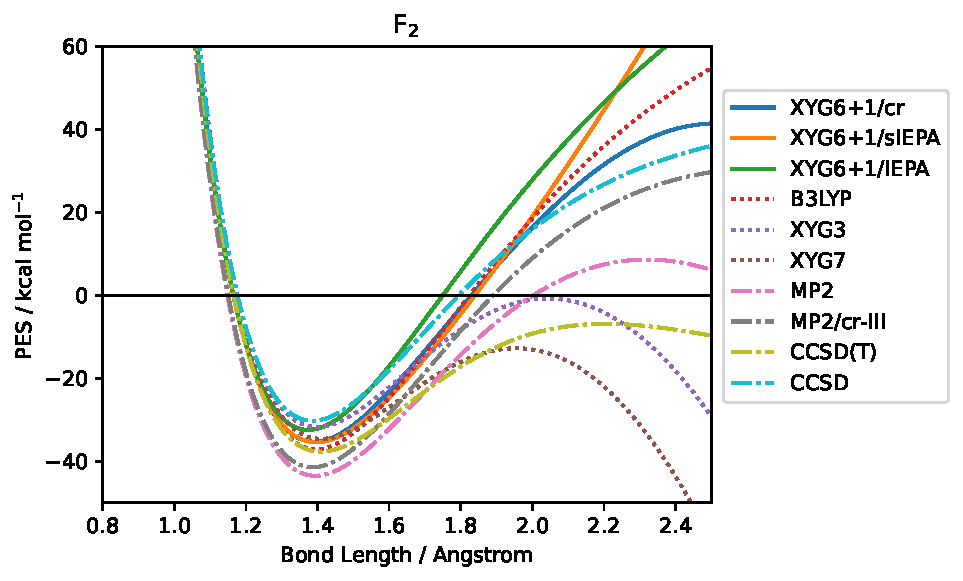
\includegraphics[width=0.7\textwidth]{assets/curve-F2.pdf}
  \caption{各方法在 \ce{F2} 解离曲线的表现。}
  \label{fig.2.curve-F2}
\end{figure}

\ce{H2O} 与 \ce{F2} 体系同样是单键解离问题。从图 \ref{fig.2.curve-H2O} 与图 \ref{fig.2.curve-H2O-part} 中可以看出,相比于 \ce{F2},各方法在 \ce{H2O} 体系上的表现明显普遍较好,但仍然存在一些问题。CCSD(T)、XYG3 方法在 2.0 \AA 以前与 DMC 的结果非常接近,但 2.0 \AA 以后显现出下降的趋势。XYG7 在解离曲线后期普遍低估能量。除 CCSD(T)、XYG$n$ ($n=3, 7$) 外的方法则对解离曲线有一定程度的高估;其中 MP2 与 XYG6+1/sIEPA 方法在 1.4--1.8 \AA 与作为参考值的 DMC 结果非常接近、其它方法则在这一段解离曲线上也稍有误差。

\begin{figure}[h]
  \centering
  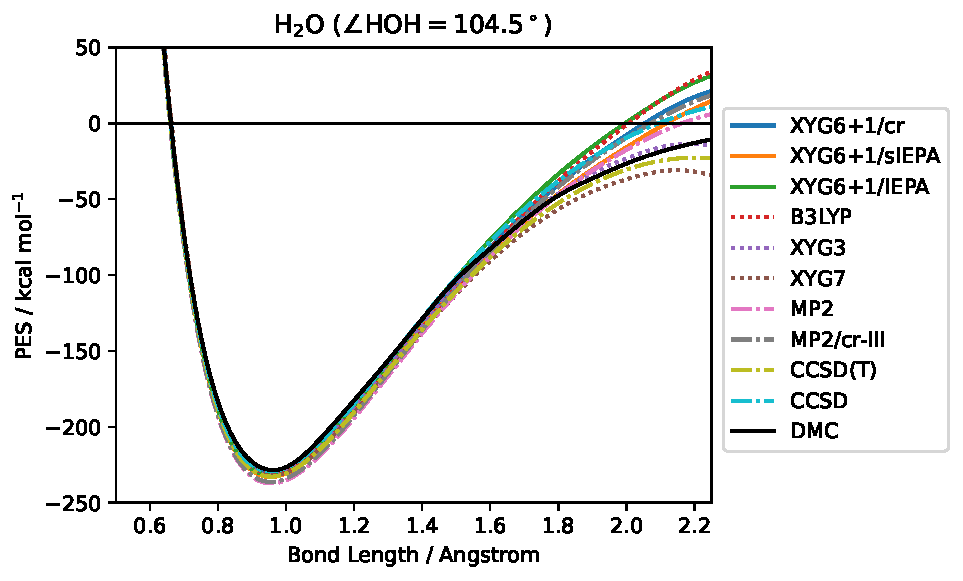
\includegraphics[width=0.7\textwidth]{assets/curve-H2O.pdf}
  \caption{各方法在 \ce{H2O} 解离曲线的表现。}
  \label{fig.2.curve-H2O}
\end{figure}

\begin{figure}[h]
  \centering
  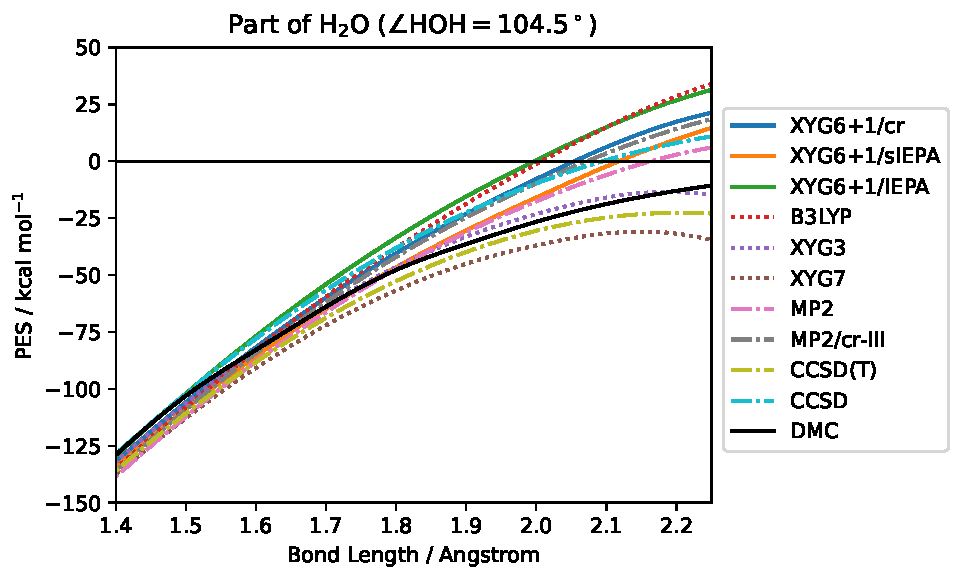
\includegraphics[width=0.7\textwidth]{assets/curve-H2O-part.pdf}
  \caption{各方法在 \ce{H2O} 解离曲线 1.4--2.25 \AA 段的表现。}
  \label{fig.2.curve-H2O-part}
\end{figure}

作为一种不太常规的单键解离问题,图 \ref{fig.2.curve-H6} 所示的环状 \ce{H6} 解离曲线也有一定挑战性。对于 CCSD 与 CCSD(T) 方法,它们在 1.8 \AA 以前的表现骄傲好,但在 2.0 \AA 以后能量明显地出现了不符合物理直觉的下降。MP2 与 MP2/cr-III 方法则不管是在 0.75--1.25 \AA 的成键区域、还是以后的解离区域,相比于参考值 DMC 都有一定程度的高估。B3LYP 在成键区域低估、但在解离区域则明显高估势能面上的能量。对于经测评的 xDH 型泛函,他们都在成键区域有良好的表现,但在解离区域产生明显的高估。

\begin{figure}[h]
  \centering
  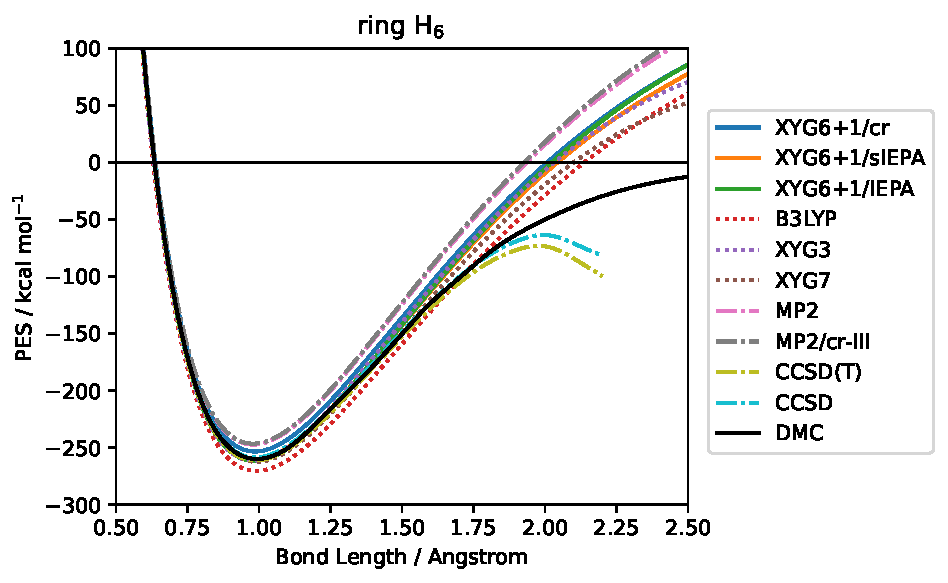
\includegraphics[width=0.7\textwidth]{assets/curve-H6.pdf}
  \caption{各方法在 \ce{H6} 解离曲线的表现。}
  \label{fig.2.curve-H6}
\end{figure}

从上述的讨论中,我们看到大多数情形下,xDH 型泛函和 CCSD、CCSD(T) 方法在成键区域的势能面与参考值非常接近。但即使是计算化学中普遍受到认可的高精度 CCSD 与 CCSD(T) 方法,在闭壳层的限制下,也难以给出定性上正确的解离曲线;而对于其它 post-HF 与密度泛函近似方法更是如此。引入 IEPA 类型相关能的诸 XYG6+1 模型可以在 \ce{N2} 问题上,相较于 XYG$n$ ($n=3,7$) 有很大程度的改善,成功地避免了解离过程中段过于严重的负误差;但正因为一般来说 IEPA 型相关能绝对值小于 MP2 相关能、并且 HOMO/LUMO gap 愈小 IEPA 型相关能与 MP2 相关能之间的差距愈大,因此绝大多数情况下诸多 XYG6+1 模型近似泛函的势能面比 XYG$n$ 模型要高。对于所有经测评的单键解离体系,相比于 DMC 参考值、或者解离极限的原子能量之和而言,XYG$n$ ($n=3,7$) 的势能面在解离区域已经有较大程度的高估;在这种情况下,正因为引入了 IEPA 型相关能,XYG6+1 模型实际上会更严重地高估势能面。因此,我们无法给出简单的结论,表明 XYG6+1 模型是否在解离曲线问题上,相比于 XYG$n$ ($n=3,7$) 是否有改善。

\section{本章小结}

在本章工作中,我们简单回顾了作为双杂化泛函理论基础的 G\"orling-Levy 微扰理论。该理论联系起 post-HF 方法与密度泛函近似。作为该微扰理论的近似,GLPT2 是诸多双杂化泛函的理论基础。GLPT2 一般由 MP2 相关能实现,而 MP2 相关能在 HOMO/LUMO gap 较小时存在明显的负误差。籍此,我们简单回顾了 IEPA 理论,并表明这些 IEPA 型相关能可以缓解 MP2 相关能在 HOMO/LUMO gap 较小情况下的误差。类似于 post-HF 框架之于 IEPA 的关系,我们对 G\"orling-Levy 微扰框架下引入 IEPA 型相关能的理论合理性作了说明。

为缓解基于 MP2 型相关能的双杂化泛函在以 \ce{N2} 解离、含过渡金属体系为代表的 HOMO/LUMO gap 较小体系上存在一定负误差的情况,同时保证在以主族反应势垒、键解离能、弱相互作用能为代表的、主流双杂化泛函表现较好的问题上保持较小的误差,我们尝试在 GMTKN55 数据集上有优异表现的 xDH@B3LYP 框架下引入 IEPA 型相关能以构造新的 XYG6+1 参数模型。在参数优化上,除了着重主族化学的 GMTKN55 外,我们引入部分含有多参考信息与过渡金属信息的 Minnesota 2015 子数据集,作参数优化得到新的泛函近似;它们依引入的相关能形式不同,称为 XYG6+1/cr、XYG6+1/IEPA 与 XYG6+1/sIEPA。

参数优化与测评结果表明,XYG6+1/cr 近似泛函在各个数据集上的表现有良好的平衡。对于 \ce{KO-}、\ce{LiO-}、\ce{Zr2} 等 HOMO/LUMO gap 小于 1.5 eV 的体系,键解离能的计算误差从 20--40 \si{kcal.mol^{-1}} 降到 10 \si{kcal.mol^{-1}} 以下,有效地降低了这类体系误差。同时,XYG6+1/cr 在 GMTKN55 数据集上的总体 WTMAD-2 误差为 2.36 \si{kcal.mol^{-1}},其表现相比于目前流行的 MP2 型相关能的双杂化泛函仍然良好;在我们所定义的 GMTKN55 和 Minnesota 2015 部分子数据集上的加权误差为 3.28 \si{kcal.mol^{-1}},是表现最优异的泛函。XYG6+1/cr 很好地平衡了主族化学问题与多参考特性或过渡金属问题的误差,基本达到了设计该泛函近似的初衷。XYG6+1/sIEPA 泛函也有类似的良好表现。

但需要承认,仅引入 IEPA 型相关能、并作关于 GMTKN55 和 Minnesota 2015 部分子数据集的优化得到的泛函,仍然存在着困难。
\begin{itemize}[nosep]
  \item 首先,HOMO/LUMO gap 小的体系一般具有多参考特性,但多参考特性的体系 HOMO/LUMO gap 不一定小;在诸如 \ce{TiCl}、\ce{NiCH2+}、\ce{VO} 为代表的多参考特性的体系上,XYG6+1 模型泛函表现较差。此外,诸如 \ce{CoH}、\ce{FeH}、\ce{FeCl} 等单参考特性含过渡金属体系的键解离也存在较大误差,而多参考特性的 MR-MGN-BE17 数据集的总的误差相当低,表明 XYG6+1 模型的误差来源与单参考或多参考的关联性不一定很强,而可能与过渡金属本身关联性稍大。
  \item 在分子解离曲线问题上,在闭壳层限制下,尽管 XYG6+1 参数模型在 \ce{N2} 体系上 2.0 \AA 以前的表现较好,但仍然无法避免解离到更远时定性不正确的趋势;而在以 \ce{F2}、\ce{H2O}、环状 \ce{H6} 为代表的单键解离问题上,不论是否引入 IEPA 或 MP2 型相关能,都在解离区域存在较大的正误差。这意味着在密度泛函近似中,仅仅矫正 MP2 相关能在 HOMO/LUMO gap 较小时的误差表现,不足以漂亮地解决解离曲线的问题。
  \item 对参数优化过程的讨论,表明严格交换能 $E_\mathrm{x}^\mathrm{exact}$ 占比愈大对 GMTKN55 主族化学问题的误差愈小、但相应地 MR-TM-BE13 等含过渡金属或多参考特性体系的数据集误差愈大;这个现象并不因为在泛函中引入 IEPA 型相关能而有所改善。同时,对于 XYG6+1 参数模型优化得到的泛函,误差容易随参与拟合数据集的变化而波动,表明该参数模型下的泛函不是非常稳健。我们无法建议将 XYG6+1 参数模型下优化的泛函,应用在 GMTKN55 与 Minnesota 2015 五个子数据集的目标化学问题以外的体系计算上。
\end{itemize}

\clearpage

\section{附录:补充数据}

\begin{table}[ht]
\centering
\caption{部分 xDH@B3LYP 模型与 XYG6+1 模型近似泛函在 MR-MGM-BE4 子集上误差。\\反应能与 MUEPB 单位 \si{kcal.mol^{-1}};HOMO/LUMO gap 单位 eV。}
\label{tab.2.supp.MR-MGM-BE4}
\widetabular{
  \begin{tabular}{ld{1.2}d{3.2}d{3.2}d{3.2}d{3.2}d{3.2}d{3.2}}
  \toprule
  \multicolumn{2}{c}{MR-MGM-BE4} & \multicolumn{3}{c}{xDH@B3LYP} & \multicolumn{3}{c}{XYG6+1\tnote{a}} \\
  \cmidrule(lr){1-2} \cmidrule(lr){3-5} \cmidrule(lr){6-8}
  System & \multicolumn{1}{c}{gap} & 
  \multicolumn{1}{c}{XYG3} & \multicolumn{1}{c}{XYG6} & \multicolumn{1}{c}{XYG7} &
  \multicolumn{1}{c}{MP2/cr} & \multicolumn{1}{c}{sIEPA} & \multicolumn{1}{c}{IEPA} \\
  \midrule
  \ce{CaO } & 2.54 & 7.01  & 8.03  & 1.50  & 1.41      & 0.18         & 0.68        \\
  \ce{KO- } & 1.03 & 38.03 & 56.57 & 46.24 & 0.00      & 0.00         & 0.00        \\
  \ce{LiO-} & 1.03 & 19.40 & 25.28 & 20.65 & 5.80      & 9.54         & 3.99        \\
  \ce{MgS } & 1.75 & -3.27 & -1.52 & -2.83 & -5.75     & -4.77        & -5.81       \\
  \midrule
  MUEPB     &      & 16.93 & 22.85 & 17.81 & 3.24      & 3.62         & 2.62        \\
  \bottomrule
  \end{tabular}
}{
  \item[a] 为方便排版,表头第二行指代的是 XYG6+1 模型泛函所使用的 IEPA 型相关能 $E_\mathrm{c}^\text{IEPA-like}$ 的具体类型;即 MP2/cr 指代 XYG6+1/cr、sIEPA 指代 XYG6+1/sIEPA、IEPA 指代 XYG6+1/IEPA。后续表格类同。
}
\end{table}

\begin{table}[ht]
\centering
\caption{部分 xDH@B3LYP 模型与 XYG6+1 模型近似泛函在 MR-MGN-BE17 子集上误差。\\反应能与 MUEPB 单位 \si{kcal.mol^{-1}};HOMO/LUMO gap 单位 eV。}
\label{tab.2.supp.MR-MGN-BE17}
\widetabular{
  \begin{tabular}{ld{2.2}d{3.2}d{3.2}d{3.2}d{3.2}d{3.2}d{3.2}}
  \toprule
  \multicolumn{2}{c}{MR-MGN-BE17} & \multicolumn{3}{c}{xDH@B3LYP} & \multicolumn{3}{c}{XYG6+1} \\
  \cmidrule(lr){1-2} \cmidrule(lr){3-5} \cmidrule(lr){6-8}
  System\tnote{a} & \multicolumn{1}{c}{gap\tnote{b}} & 
  \multicolumn{1}{c}{XYG3} & \multicolumn{1}{c}{XYG6} & \multicolumn{1}{c}{XYG7} &
  \multicolumn{1}{c}{MP2/cr} & \multicolumn{1}{c}{sIEPA} & \multicolumn{1}{c}{IEPA} \\
  \midrule
  \ce{NF3 }          &  10.08 & -2.57 & -0.70 & -1.54 & -0.60     & -0.89        & -1.13       \\
  \ce{CO2 }          &  9.87  & -0.40 & 1.84  & -0.25 & 0.61      & 0.42         & -0.12       \\
  \ce{SiO }          &  6.34  & 1.65  & 3.88  & 1.26  & -0.22     & 0.00         & -2.69       \\
  \ce{SO2 }          &  5.69  & -1.34 & 1.50  & -0.71 & -0.84     & -0.99        & -2.35       \\
  \ce{CO2 }          &  9.41  & -1.06 & 1.84  & -0.11 & -0.25     & 0.10         & -2.29       \\
  \ce{SO2 }          &  3.69  & 0.29  & 0.41  & -0.87 & -1.46     & -3.63        & -1.81       \\
  \ce{ClO }          &  2.78  & -1.94 & -0.71 & -1.48 & -1.95     & -3.02        & -2.43       \\
  \ce{F2  }          &  7.23  & -6.91 & -2.23 & -4.17 & -3.35     & -3.28        & -6.35       \\
  \ce{N2  }          &  10.99 & 1.17  & 2.60  & 2.31  & -1.35     & 1.97         & -3.23       \\
  \ce{O2  }          &  5.28  & -1.09 & -1.29 & -1.67 & -2.65     & -7.06        & -3.60       \\
  \ce{NO  }          &  3.01  & -0.43 & 1.33  & 0.77  & -1.27     & -0.43        & -3.02       \\
  \ce{CN  }          &  3.58  & 2.82  & 5.52  & 3.05  & -0.28     & 0.89         & -3.54       \\
  \ce{B2  }          &  2.17  & -1.12 & 2.16  & -0.67 & -5.74     & -9.10        & -7.72       \\
  \ce{O3  }\tnote{c} &  4.12  & 0.30  & 13.49 & 8.35  & 0.06      & 3.59         & -7.78       \\
  \ce{C2  }          &  1.80  & 4.19  & 17.97 & 10.48 & -5.59     & -2.42        & -15.25      \\
  \ce{S4  }\tnote{d} &  2.28  & 1.56  & 9.44  & 6.47  & -1.59     & 2.84         & -2.51       \\
  \ce{Cl2O}\tnote{e} &  4.31  & -1.98 & 0.60  & -0.61 & -0.29     & -0.45        & -1.64       \\
  \midrule
  MUEPB              &        & 1.81  & 3.97  & 2.63  & 1.65      & 2.42         & 3.97        \\
  \bottomrule
  \end{tabular}
}{
  \item[a] 对于未标明化学反应式的体系,其对应的反应是原子化反应。后续表格类同。
  \item[b] 对于开壳层体系,HOMO/LUMO gap 是通过 $\alpha, \beta$ 两种自旋的 HOMO 最大值与 LUMO 最小值的差减计算得到。后续表格类同。
  \item[c] \ce{O3 -> O2 + O}
  \item[d] \ce{S4 -> 2 S2}
  \item[e] \ce{Cl2O -> Cl2 + O}
}
\end{table}

\begin{table}[ht]
\centering
\caption{部分 xDH@B3LYP 模型与 XYG6+1 模型近似泛函在 MR-TM-BE13 子集上误差。\\反应能与 MUEPB 单位 \si{kcal.mol^{-1}};HOMO/LUMO gap 单位 eV。}
\label{tab.2.supp.MR-TM-BE13}
\widetabular{
  \begin{tabular}{ld{1.2}d{3.2}d{3.2}d{3.2}d{3.2}d{3.2}d{3.2}}
  \toprule
  \multicolumn{2}{c}{MR-TM-BE13} & \multicolumn{3}{c}{xDH@B3LYP} & \multicolumn{3}{c}{XYG6+1} \\
  \cmidrule(lr){1-2} \cmidrule(lr){3-5} \cmidrule(lr){6-8}
  System & \multicolumn{1}{c}{gap} & 
  \multicolumn{1}{c}{XYG3} & \multicolumn{1}{c}{XYG6} & \multicolumn{1}{c}{XYG7} &
  \multicolumn{1}{c}{MP2/cr} & \multicolumn{1}{c}{sIEPA} & \multicolumn{1}{c}{IEPA} \\
  \midrule
  \ce{TiCl    }          & 5.72 & -10.78 & -13.28 & -15.27 & -12.64    & -18.46       & -10.47      \\
  \ce{VF5     }          & 5.94 & 5.37   & 9.00   & 6.49   & 5.15      & 3.76         & 0.96        \\
  \ce{CrCl    }          & 2.93 & 3.09   & 3.13   & 3.18   & 1.10      & 2.35         & 0.69        \\
  \ce{CrOF    }          & 1.68 & -5.09  & 0.04   & -3.31  & -6.61     & -4.28        & -11.81      \\
  \ce{(FeBr2)2}          & 2.73 & 8.23   & 9.72   & 10.04  & 8.49      & 8.91         & 8.22        \\
  \ce{Co(CO)4H}          & 5.89 & 20.39  & 27.69  & 23.02  & 13.45     & 13.98        & 8.34        \\
  \ce{NiCH2+  }\tnote{a} & 3.90 & 18.44  & 20.94  & 18.52  & 12.16     & 8.34         & 8.73        \\
  \ce{FeCO5   }\tnote{b} & 4.96 & 24.37  & 29.99  & 26.32  & 12.90     & 15.84        & 11.56       \\
  \ce{VS      }          & 2.90 & 14.57  & 17.19  & 15.79  & 3.69      & 3.25         & -0.99       \\
  \ce{CuCl    }          & 3.99 & 1.28   & 3.15   & 2.59   & 1.21      & 1.81         & 0.75        \\
  \ce{CuH     }          & 4.23 & 2.29   & 2.91   & 3.57   & 0.97      & 2.20         & 0.33        \\
  \ce{NiCl    }          & 3.14 & 4.75   & 6.76   & 5.81   & 4.17      & 4.08         & 2.89        \\
  \ce{VO      }          & 2.55 & 20.04  & 27.78  & 23.64  & 13.58     & 13.49        & 3.22        \\
  \midrule
  MUEPB                  &      & 10.67  & 13.20  & 12.12  & 7.40      & 7.75         & 5.30        \\
  \bottomrule
  \end{tabular}
}{
  \item[a] \ce{NiCH2+ -> Ni+ + CH2}
  \item[b] \ce{FeCO5 -> Fe + 5CO}
}
\end{table}

\begin{table}[ht]
\centering
\caption{部分 xDH@B3LYP 模型与 XYG6+1 模型近似泛函在 SR-MGM-BE9 子集上误差。\\反应能与 MUEPB 单位 \si{kcal.mol^{-1}};HOMO/LUMO gap 单位 eV。}
\label{tab.2.supp.SR-MGM-BE9}
\widetabular{
  \begin{tabular}{ld{1.2}d{3.2}d{3.2}d{3.2}d{3.2}d{3.2}d{3.2}}
  \toprule
  \multicolumn{2}{c}{SR-MGM-BE9} & \multicolumn{3}{c}{xDH@B3LYP} & \multicolumn{3}{c}{XYG6+1} \\
  \cmidrule(lr){1-2} \cmidrule(lr){3-5} \cmidrule(lr){6-8}
  System & \multicolumn{1}{c}{gap} & 
                 \multicolumn{1}{c}{XYG3} & \multicolumn{1}{c}{XYG6} & \multicolumn{1}{c}{XYG7} &
                 \multicolumn{1}{c}{MP2/cr} & \multicolumn{1}{c}{sIEPA} & \multicolumn{1}{c}{IEPA} \\
  \midrule
  \ce{AlCl3}          & 7.35 & 0.02  & 0.72  & -0.07 & -0.11     & 0.29         & 0.55        \\
  \ce{AlF3 }          & 9.43 & -1.23 & -0.30 & -3.03 & -0.74     & -1.39        & -1.18       \\
  \ce{KOH  }\tnote{a} & 3.72 & -1.73 & -0.79 & -3.14 & -2.71     & -2.55        & -3.59       \\
  \ce{NaO  }          & 3.09 & -2.18 & -2.62 & -4.22 & -4.25     & -3.79        & -4.47       \\
  \ce{LiO  }          & 3.41 & 1.83  & 0.52  & -0.92 & -0.72     & -0.12        & -0.03       \\
  \ce{LiCl }          & 5.31 & -0.87 & -1.58 & -2.43 & -2.99     & -2.17        & -2.00       \\
  \ce{AlCl3}          & 5.01 & -0.05 & 0.39  & -0.26 & -0.81     & -0.39        & -0.32       \\
  \ce{ZnSe }          & 1.64 & 6.16  & 7.86  & 7.89  & 4.51      & 5.43         & 4.55        \\
  \ce{ZnCl }          & 2.34 & 0.25  & 1.22  & 0.97  & 0.93      & 0.75         & 1.54        \\
  \midrule
  MUEPB              &      & 1.59  & 1.78  & 2.55  & 1.97      & 1.87         & 2.03        \\
  \bottomrule
  \end{tabular}
}{
  \item[a] \ce{KOH -> K + OH}
}
\end{table}

\begin{table}[ht]
\centering
\caption{部分 xDH@B3LYP 模型与 XYG6+1 模型近似泛函在 SR-TM-BE17 子集上误差。\\反应能与 MUEPB 单位 \si{kcal.mol^{-1}};HOMO/LUMO gap 单位 eV。}
\label{tab.2.supp.SR-TM-BE17}
\widetabular{
  \begin{tabular}{ld{1.2}d{3.2}d{3.2}d{3.2}d{3.2}d{3.2}d{3.2}}
  \toprule
  \multicolumn{2}{c}{SR-TM-BE17} & \multicolumn{3}{c}{xDH@B3LYP} & \multicolumn{3}{c}{XYG6+1} \\
  \cmidrule(lr){1-2} \cmidrule(lr){3-5} \cmidrule(lr){6-8}
  System & \multicolumn{1}{c}{gap} & 
                 \multicolumn{1}{c}{XYG3} & \multicolumn{1}{c}{XYG6} & \multicolumn{1}{c}{XYG7} &
                 \multicolumn{1}{c}{MP2/cr} & \multicolumn{1}{c}{sIEPA} & \multicolumn{1}{c}{IEPA} \\
  \midrule
  \ce{CrCl2           }          & 2.60 & 1.40  & 3.42  & 3.43  & 1.60      & 5.75         & 1.47        \\
  \ce{MnF2            }          & 5.12 & 2.27  & 3.63  & 0.51  & 3.28      & 1.43         & 1.76        \\
  \ce{FeCl2           }          & 2.93 & 5.41  & 7.02  & 7.75  & 5.57      & 6.11         & 5.36        \\
  \ce{CoCl2           }          & 3.16 & -1.54 & -0.79 & -0.27 & -2.80     & -3.80        & -2.89       \\
  \ce{Ag2             }          & 3.00 & 0.11  & 1.25  & 1.00  & -0.79     & -0.34        & -0.91       \\
  \ce{AgH             }          & 4.34 & 0.67  & 0.90  & 2.14  & -0.14     & 1.53         & 0.50        \\
  \ce{CoH             }          & 3.05 & 17.76 & 18.57 & 19.38 & 16.23     & 18.28        & 15.57       \\
  \ce{CrCH3+          }\tnote{a} & 3.49 & 3.52  & 5.06  & 5.93  & 3.78      & 5.04         & 2.89        \\
  \ce{Cu2             }          & 3.33 & -0.46 & 1.09  & 0.28  & -2.30     & -2.14        & -3.27       \\
  \ce{CuAg            }          & 3.35 & 0.10  & 1.61  & 0.89  & -0.96     & -0.84        & -1.93       \\
  \ce{CuH2O+          }\tnote{b} & 5.01 & 0.12  & 0.81  & 0.56  & 0.49      & -0.44        & 0.04        \\
  \ce{FeH             }          & 2.40 & 25.16 & 26.43 & 27.30 & 23.81     & 26.57        & 23.07       \\
  \ce{VCO+            }\tnote{c} & 2.52 & -1.99 & -4.30 & -3.33 & -4.60     & -8.32        & -3.79       \\
  \ce{Zr2             }          & 1.34 & 23.14 & 27.10 & 19.22 & 0.34      & -0.21        & -0.03       \\
  \ce{Pd(PH3)2(C6H8)  }\tnote{d} & 4.32 & 1.23  & 4.18  & 4.35  & 2.01      & 0.80         & -0.04       \\
  \ce{Pd(PH3)2(C10H12)}\tnote{e} & 4.19 & 0.29  & 4.51  & 4.62  & 1.86      & 0.21         & -1.86       \\
  \ce{FeCl            }          & 1.53 & 9.30  & 12.17 & 13.86 & 12.05     & 13.53        & 12.69       \\
  \midrule
  \ce{MUEPB           }          &      & 5.56  & 7.23  & 6.75  & 4.86      & 5.61         & 4.59        \\
  \bottomrule
  \end{tabular}
}{
  \item[a] \ce{CrCH3+ -> Cr+ + CH3}
  \item[b] \ce{CuH2O+ -> Cu+ + H2O}
  \item[c] \ce{VCO+ -> V+ + CO}
  \item[d] \ce{Pd(PH3)2(C6H8) -> Pd(PH3)2 + C6H8}
  \item[e] \ce{Pd(PH3)2(C10H12) -> Pd(PH3)2 + C10H12}
}
\end{table}

\clearpage

\begin{ThreePartTable}
\begin{longtable}{lld{2.2}d{2.2}d{2.2}d{2.2}d{2.2}d{2.2}}
  \caption{部分 xDH@B3LYP 模型与 XYG6+1 模型近似泛函在 SR-TM-BE17 子集上误差。\\小子集误差以 MAD 为量标,子集与总误差以 WTMAD-2 为量标,单位 \si{kcal.mol^{-1}}。}
  \label{tab.2.supp.GMTKN55}
  \\ \toprule
  \multicolumn{2}{c}{GMTKN55} & \multicolumn{3}{c}{xDH@B3LYP} & \multicolumn{3}{c}{XYG6+1} \\
  \cmidrule(lr){1-2} \cmidrule(lr){3-5} \cmidrule(lr){6-8}
  Subset  & Dataset   & \multicolumn{1}{c}{XYG3}  & \multicolumn{1}{c}{XYG6}  & \multicolumn{1}{c}{XYG7}  & \multicolumn{1}{c}{MP2/cr} & \multicolumn{1}{c}{sIEPA} & \multicolumn{1}{c}{IEPA}  \\ \midrule
  \endfirsthead
  \caption{(续表)}
  \\ \toprule
  \multicolumn{2}{c}{GMTKN55} & \multicolumn{3}{c}{xDH@B3LYP} & \multicolumn{3}{c}{XYG6+1} \\
  \cmidrule(lr){1-2} \cmidrule(lr){3-5} \cmidrule(lr){6-8}
  Subset  & Dataset   & \multicolumn{1}{c}{XYG3}  & \multicolumn{1}{c}{XYG6}  & \multicolumn{1}{c}{XYG7}  & \multicolumn{1}{c}{MP2/cr} & \multicolumn{1}{c}{sIEPA} & \multicolumn{1}{c}{IEPA}  \\ \midrule
  \endhead
  %
  Sub1    & W4-11     & 2.52  & 2.08  & 2.36  & 3.24   & 2.61  & 3.03  \\
          & G21EA     & 2.01  & 1.81  & 1.27  & 2.91   & 1.70  & 1.50  \\
          & G21IP     & 1.39  & 1.44  & 1.92  & 2.19   & 1.85  & 3.11  \\
          & DIPCS10   & 2.20  & 2.23  & 4.52  & 4.59   & 1.82  & 4.36  \\
          & PA26      & 0.97  & 0.82  & 1.86  & 0.80   & 1.04  & 1.11  \\
          & SIE4x4    & 2.43  & 0.48  & 0.56  & 0.56   & 0.87  & 3.59  \\
          & ALKBDE10  & 3.60  & 4.58  & 4.36  & 2.96   & 2.83  & 3.33  \\
          & YBDE18    & 1.06  & 1.33  & 0.73  & 0.67   & 1.49  & 0.70  \\
          & AL2X6     & 2.29  & 0.72  & 0.84  & 0.99   & 0.76  & 1.12  \\
          & HEAVYSB11 & 1.47  & 1.31  & 1.40  & 1.17   & 1.12  & 1.07  \\
          & NBPRC     & 1.42  & 0.57  & 0.64  & 0.88   & 1.42  & 1.66  \\
          & ALK8      & 1.33  & 2.11  & 1.82  & 1.24   & 2.02  & 1.21  \\
          & RC21      & 0.80  & 0.97  & 0.81  & 0.65   & 0.93  & 1.70  \\
          & G2RC      & 1.28  & 1.42  & 1.50  & 1.38   & 1.90  & 3.49  \\
          & BH76RC    & 1.03  & 0.93  & 0.86  & 0.90   & 0.93  & 1.15  \\
          & FH51      & 1.09  & 0.87  & 0.71  & 1.03   & 1.30  & 1.75  \\
          & TAUT15    & 0.49  & 0.56  & 0.38  & 0.49   & 0.69  & 0.58  \\
          & DC13      & 5.70  & 4.26  & 3.32  & 1.98   & 1.86  & 2.91  \\ \hdashline
  Sub2    & MB16-43   & 24.12 & 17.85 & 23.55 & 17.06  & 22.47 & 18.13 \\
          & DARC      & 2.82  & 0.64  & 0.59  & 1.19   & 2.03  & 1.32  \\
          & RSE43     & 0.25  & 0.24  & 0.21  & 0.22   & 0.47  & 0.22  \\
          & BSR36     & 2.12  & 0.45  & 0.39  & 1.19   & 2.55  & 3.44  \\
          & CDIE20    & 0.49  & 0.19  & 0.17  & 0.20   & 0.32  & 0.41  \\
          & ISO34     & 0.80  & 0.43  & 0.40  & 0.42   & 0.53  & 0.63  \\
          & ISOL24    & 2.67  & 1.20  & 1.07  & 0.95   & 0.87  & 1.67  \\
          & C60ISO    & 9.86  & 13.07 & 11.15 & 1.78   & 4.79  & 3.19  \\
          & PArel     & 0.56  & 0.41  & 0.40  & 0.40   & 0.35  & 0.62  \\ \hdashline
  Sub3    & BH76      & 0.71  & 1.02  & 0.69  & 0.75   & 1.33  & 0.82  \\
          & BHPERI    & 0.59  & 0.45  & 0.55  & 1.15   & 2.37  & 1.09  \\
          & BHDIV10   & 1.40  & 1.06  & 0.87  & 1.03   & 1.44  & 1.08  \\
          & INV24     & 0.68  & 0.62  & 0.66  & 0.84   & 0.99  & 1.11  \\
          & BHROT27   & 0.20  & 0.16  & 0.14  & 0.24   & 0.23  & 0.34  \\
          & PX13      & 0.50  & 0.93  & 1.39  & 1.43   & 0.92  & 1.81  \\
          & WCPT18    & 0.66  & 1.41  & 1.75  & 1.19   & 0.82  & 1.62  \\ \hdashline
  Sub4    & RG18      & 0.15  & 0.07  & 0.08  & 0.08   & 0.09  & 0.29  \\
          & ADIM6     & 1.24  & 0.42  & 0.35  & 0.67   & 0.65  & 0.84  \\
          & S22       & 0.57  & 0.14  & 0.14  & 0.35   & 0.37  & 0.77  \\
          & S66       & 0.60  & 0.21  & 0.18  & 0.37   & 0.38  & 0.68  \\
          & HEAVY28   & 0.19  & 0.12  & 0.15  & 0.08   & 0.12  & 0.16  \\
          & WATER27   & 1.01  & 2.15  & 2.41  & 2.60   & 3.61  & 7.02  \\
          & CARBHB12  & 0.24  & 0.26  & 0.23  & 0.28   & 0.31  & 0.70  \\
          & PNICO23   & 0.38  & 0.11  & 0.09  & 0.19   & 0.24  & 0.39  \\
          & HAL59     & 0.30  & 0.33  & 0.30  & 0.31   & 0.28  & 0.41  \\
          & AHB21     & 0.39  & 0.39  & 0.40  & 0.36   & 0.56  & 1.21  \\
          & CHB6      & 1.26  & 1.14  & 1.00  & 1.28   & 1.52  & 1.49  \\
          & IL16      & 0.87  & 0.32  & 0.80  & 0.47   & 0.41  & 0.37  \\ \hdashline
  Sub5    & IDISP     & 2.73  & 0.51  & 0.49  & 1.09   & 1.47  & 3.18  \\
          & ICONF     & 0.25  & 0.12  & 0.11  & 0.13   & 0.12  & 0.26  \\
          & ACONF     & 0.24  & 0.08  & 0.08  & 0.09   & 0.14  & 0.25  \\
          & Amino20x4 & 0.15  & 0.08  & 0.07  & 0.09   & 0.13  & 0.24  \\
          & PCONF21   & 0.56  & 0.17  & 0.14  & 0.28   & 0.38  & 1.04  \\
          & MCONF     & 0.21  & 0.31  & 0.25  & 0.15   & 0.13  & 0.38  \\
          & SCONF     & 0.10  & 0.11  & 0.12  & 0.09   & 0.10  & 0.10  \\
          & UPU23     & 0.55  & 0.37  & 0.37  & 0.43   & 0.52  & 0.75  \\
          & BUT14DIOL & 0.07  & 0.05  & 0.04  & 0.08   & 0.06  & 0.11  \\ \midrule
  WTMAD-2 & Sub1      & 1.74  & 1.50  & 1.29  & 1.53   & 1.69  & 2.10  \\
          & Sub2      & 4.70  & 2.45  & 2.38  & 2.54   & 3.97  & 4.53  \\
          & Sub3      & 1.71  & 2.11  & 1.82  & 2.22   & 3.28  & 2.57  \\
          & Sub4      & 5.15  & 2.83  & 2.86  & 3.38   & 3.70  & 6.97  \\
          & Sub5      & 4.25  & 2.43  & 2.10  & 2.59   & 3.11  & 6.60  \\
          & All       & 3.39  & 2.18  & 2.01  & 2.36   & 2.94  & 4.41  \\ \bottomrule
\end{longtable}
\end{ThreePartTable}

\begin{figure}[h]
  \centering
  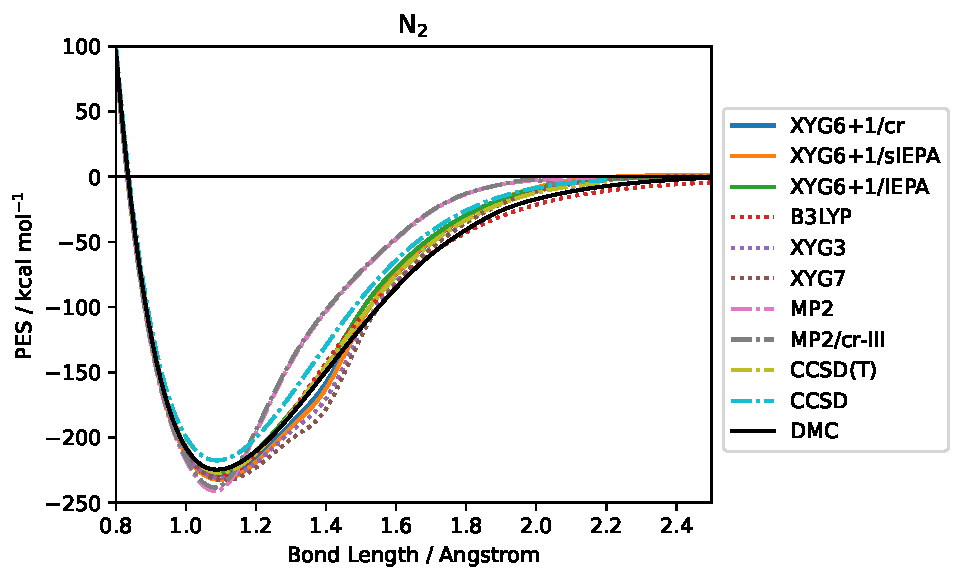
\includegraphics[width=0.7\textwidth]{assets/curve-N2-stab.pdf}
  \caption{各方法在 \ce{N2} 解离曲线的表现。参考态方法均在开壳层下优化到稳定。}
  \label{fig.2.curve-N2-stab}
\end{figure}

\begin{figure}[h]
  \centering
  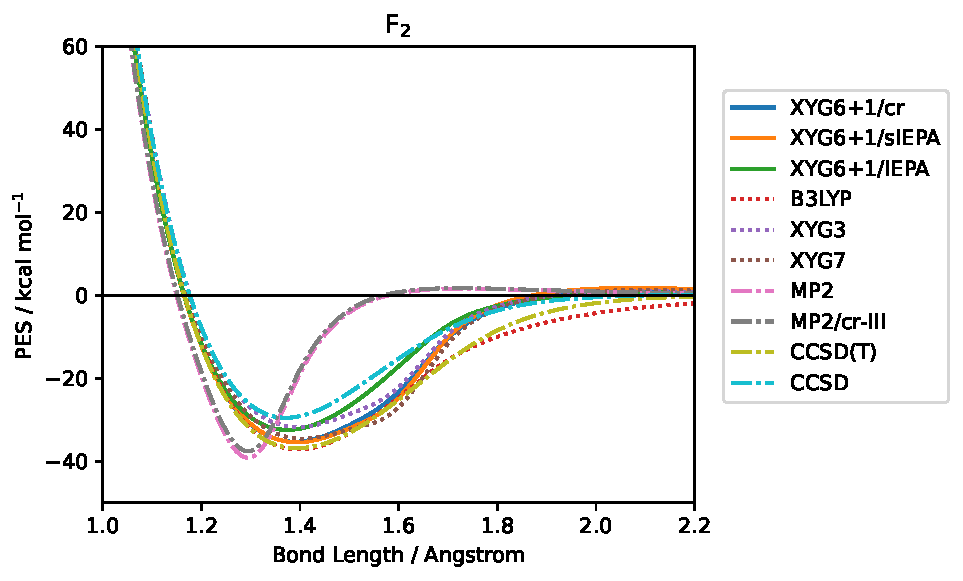
\includegraphics[width=0.7\textwidth]{assets/curve-F2-stab.pdf}
  \caption{各方法在 \ce{F2} 解离曲线的表现。参考态方法均在开壳层下优化到稳定。}
  \label{fig.2.curve-F2-stab}
\end{figure}

\begin{figure}[h]
  \centering
  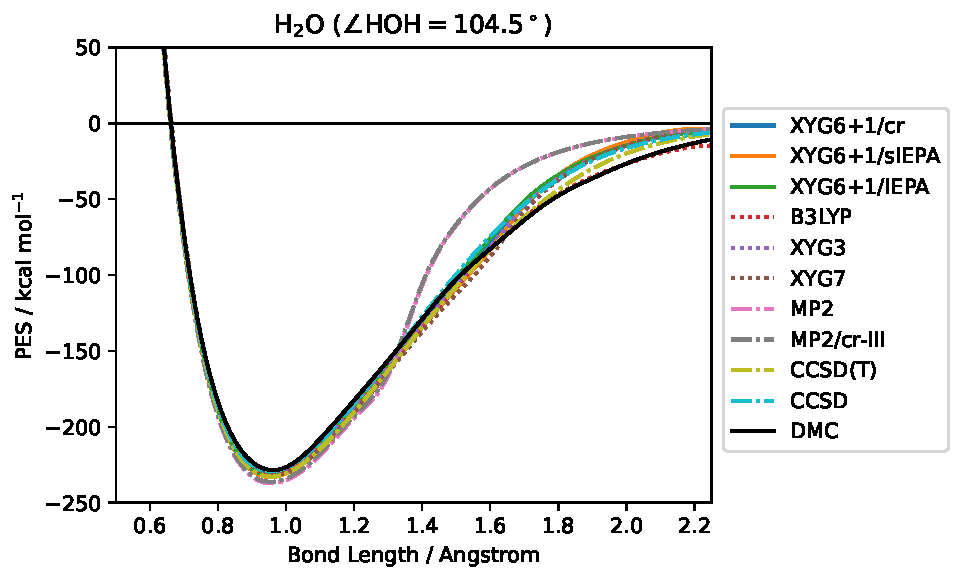
\includegraphics[width=0.7\textwidth]{assets/curve-H2O-stab.pdf}
  \caption{各方法在 \ce{H2O} 解离曲线的表现。参考态方法均在开壳层下优化到稳定。}
  \label{fig.2.curve-H2O-stab}
\end{figure}

\begin{figure}[h]
  \centering
  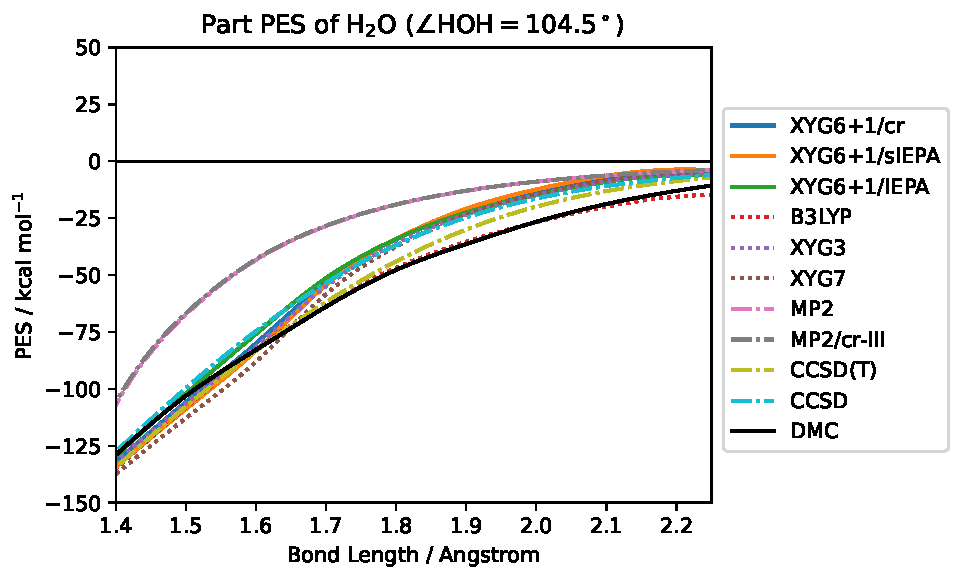
\includegraphics[width=0.7\textwidth]{assets/curve-H2O-part-stab.pdf}
  \caption{各方法在 \ce{H2O} 解离曲线 1.4--2.25 \AA 段的表现。参考态方法均在开壳层下优化到稳定。}
  \label{fig.2.curve-H2O-part-stab}
\end{figure}

\begin{figure}[h]
  \centering
  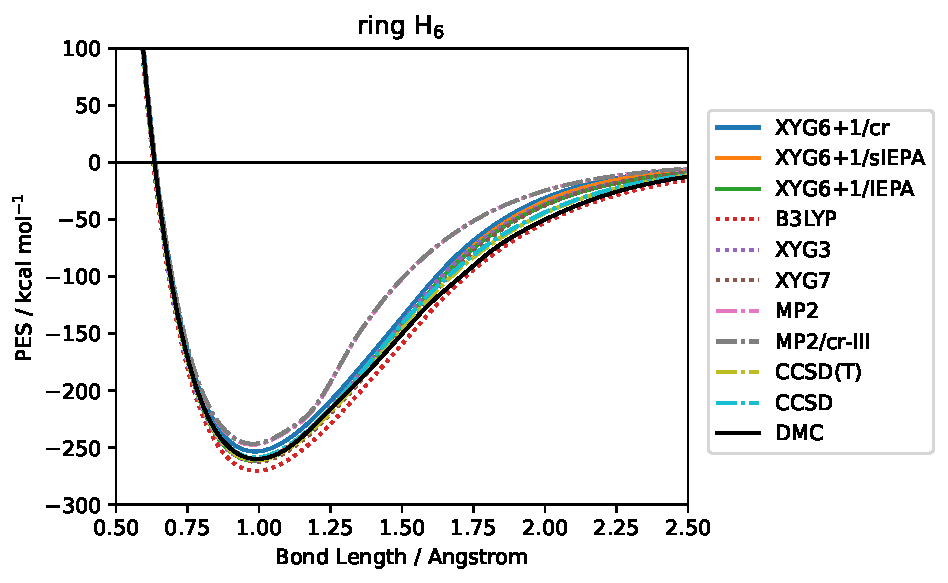
\includegraphics[width=0.7\textwidth]{assets/curve-H6-stab.pdf}
  \caption{各方法在 \ce{H6} 解离曲线的表现。参考态方法均在开壳层下优化到稳定。}
  \label{fig.2.curve-H6-stab}
\end{figure}

\newpage

\section{附录:电子对方法的前置理论}

\subsection{组态相互作用方法 CI}

电子对方法来源于精确波函数方法的近似。这里将简要地回顾两类典型的波函数方法:组态相互作用方法 CI 与耦合簇方法 CC。

Hartree-Fock 参考态与 Hartree-Fock 算符下的激发态所构成的函数空间,可以认为是完备的多电子波函数。CI 方法的思路是在这个完备的函数空间下,对分子体系的Hamilton 算符 $\hat H$ 求取变分极小以获得基态能量。若 Hartree-Fock 基态记为 $| 0 \rangle$\footnote{出于讨论简化,仅考虑 Hartree-Fock 基态非简并的情形,且所有占据、非占轨道相互正交 (即满足 canonical Hartree-Fock 条件)。}、占据轨道角标为 $i, j, k, l, \cdots$、非占轨道角标为 $a, b, c, d, \cdots$,那么 Hartree-Fock 算符下的激发态可以表示为
\begin{equation}
  | {}_{ijk\cdots}^{abc\cdots} \rangle = a_a^\dagger a_b^\dagger a_c^\dagger \cdots a_k a_j a_i | 0 \rangle
\end{equation}
上式中的 $a_i$ 与 $a_a^\dagger$ 分别代表对占据轨道 $i$ 的湮灭算符与对非占轨道 $a$ 的生成算符。那么,令 CI 波函数为
\begin{align}
  | \Psi^\text{CI} \rangle &= | 0 \rangle + \hat C_1 | 0 \rangle + \hat C_2 | 0 \rangle + \hat C_3 | 0 \rangle + \cdots \notag\\
  &= | 0 \rangle + \sum_{ia} c_i^a a_a^\dagger a_i | 0 \rangle + \sum_{ijab} c_{ij}^{ab} a_a^\dagger a_b^\dagger a_j a_i | 0 \rangle + \sum_{ijkabc} c_{ijk}^{abc} a_a^\dagger a_b^\dagger a_c^\dagger a_k a_j a_i | 0 \rangle + \cdots \notag\\
  &= | 0 \rangle + \sum_{ia} c_i^a | {}_i^a \rangle + \sum_{ijab} c_{ij}^{ab} | {}_{ij}^{ab} \rangle  + \sum_{ijkabc} c_{ijk}^{abc} | {}_{ijk}^{abc} \rangle + \cdots
\end{align}
其中,上式的 $\hat C_1, \hat C_2, \hat C_3, \cdots$ 表示 Hartree-Fock 算符下的一次、二次、三次等激发算符;$c_i^a, c_{ij}^{ab}, c_{ijk}^{abc}, \cdots$ 为 CI 波函数 $| \Psi^\text{CI} \rangle$ 的变分系数\footnote{记号不严谨。我们经常用 $c_{ij}^{ab}$ 表示所有二次激发系数的集合 $\{ c_{ij}^{ab} \}_{ijab}$;但为表达式简洁,就仅用其中一个系数代表所有激发系数集合。对于一次、三次等其它阶次激发同理。}:
\begin{equation}
  \label{eq.2.CI-variation}
  E_\mathrm{c}^\mathrm{CI} = \min_{c_i^a, c_{ij}^{ab}, c_{ijk}^{abc}, \cdots} \frac{\langle \Psi^\mathrm{CI} | \hat H - E_0 | \Psi^\mathrm{CI} \rangle}{\langle \Psi^\mathrm{CI} | \Psi^\mathrm{CI} \rangle}
\end{equation}
其中,$E_0 = \langle 0 | \hat H | 0 \rangle$ 表示 Hartree-Fock 基态能量。

若将所有 Hartree-Fock 的激发态系数纳入变分计算,则称为 Full-CI 方法。Full-CI 的计算量为大约是基函数的阶乘 $O(C_{n_\mathrm{basis}}^{n_\mathrm{occ}})$,对于实际分子体系是不可接受的。如果不考虑三次或以上 Hartree-Fock 激发态,那么该方法称为 CISD;若进一步地,由 Brillouin 定理的推论,单次和三次 Hartree-Fock 激发态对波函数的贡献较小,从而可以将 $c_i^a$ 近似为零,则该方法称为 CID:
\begin{align}
  | \Psi^\text{CID} \rangle &= | 0 \rangle + \sum_{ijab} c_{ij}^{ab} | {}_{ij}^{ab} \rangle \\
  E_\mathrm{c}^\mathrm{CID} &= \min_{c_i^a, c_{ij}^{ab}} \frac{\langle \Psi^\mathrm{CID} | \hat H - E_0 | \Psi^\mathrm{CID} \rangle}{\langle \Psi^\mathrm{CID} | \Psi^\mathrm{CID} \rangle}
\end{align}
类似地,若仅考虑贡献较大的二次与四次 Hartree-Fock 激发态,那么该方法称为 CIDQ。这类以排除特定 Hartree-Fock 激发次数的 CI 近似方法称为截断的 CI (Truncated CI)。在后文中,我们经常将二次与四次 Hartree-Fock 激发态记为 $| \chi_\mathrm{D} \rangle$ 与 $| \chi_\mathrm{Q} \rangle$:
\begin{align}
  \label{eq.2.ci-chi-d}
  | \chi_\mathrm{D} \rangle &= \sum_{ijab} c_{ij}^{ab} | {}_{ij}^{ab} \rangle \\
  \label{eq.2.ci-chi-q}
  | \chi_\mathrm{Q} \rangle &= \sum_{ijklabcd} c_{ijkl}^{abcd} | {}_{ijkl}^{abcd} \rangle
\end{align}
那么,对于 CID 与 CIDQ 近似,式 (\ref{eq.2.CI-variation}) 所表示的变分条件可以转化为下述的本征方程\footnote{记号不严谨。需要注意到,CID 与 CIDQ 的变分条件并不相同,因此 CID 方法下的 $\chi_\mathrm{D}$ 与 CIDQ 方法下的 $\chi_\mathrm{D}$ 的激发系数 $c_{ij}^{ab}$ 并不相同。出于公式的表达简洁,我们不会在 $\chi_\mathrm{D}$ 或 $\chi_\mathrm{Q}$ 上标具体的方法近似。后文的其它波函数近似方法也存在类似记号。}:
\begin{align}
  \label{eq.2.CID-eigen}
  (\hat H - E_0) | 0 + \chi_\mathrm{D} \rangle &= E_\mathrm{c}^\mathrm{CID} | 0 + \chi_\mathrm{D} \rangle \quad \text{(CID)} \\
  \label{eq.2.CIDQ-eigen}
  (\hat H - E_0) | 0 + \chi_\mathrm{D} + \chi_\mathrm{Q} \rangle &= E_\mathrm{c}^\mathrm{CIDQ} | 0 + \chi_\mathrm{D} + \chi_\mathrm{Q} \rangle \quad \text{(CIDQ)}
\end{align}

需要指出,这类截断的 CI 近似能量满足轨道正交变换的不变性 (unitary invariance),但不满足大小延展性 (size extensivity)。以独立 \ce{He}$_{N}$ 体系为例,CID 相关能随体系中 \ce{He} 原子的数量 $N$ 增加而表现为非线性的渐进性质\cite{Ahlrichs-Ahlrichs.CPC.1979, Szabo-Ostlund.Dover.1996}:
\begin{equation}
  E_\mathrm{c}^\mathrm{CID} \propto \sqrt{N}
\end{equation}
这意味着,截断的 CI 方法在较大的体系下,其相关能存在非常严重的正误差。而同时,CID 方法的计算量为 $O(n_\mathrm{occ}^2 n_\mathrm{vir}^4)$,即六次方标度,相比于 Hartree-Fock 或 MP2 是非常巨大的计算消耗。因此,这类截断的 CI 方法并非在计算量与精度上有很好的平衡。但同时,CI 理论非常简洁明了,因此它是几乎所有 post-HF 方法的理论基础。

\subsection{耦合簇方法 CC}

CC 理论来源于核物理问题\cite{Coester-Coester.NPB.1958,Coester-Kuemmel.NPB.1960},而后引入到化学问题中\cite{Cizek-Cizek.JCP.1966, Cizek-Paldus.IJQC.1971}。与 CI 方法针对激发算符 $\hat C_1, \hat C_2, \cdots$ 对应的激发系数 $c_i^a, c_{ij}^{ab}$ 进行变分优化不同,一方面,CC 方法的波函数是通过簇算符给出:
\begin{gather}
  \hat T = \hat T_1 + \hat T_2 + \cdots = \sum_{ia} t_i^a a_a^\dagger a_i + \sum_{ij}^{ab} a_a^\dagger a_b^\dagger a_j a_i + \cdots \\
  | \Psi^\text{CC} \rangle = \mathrm{e}^{\hat T} | 0 \rangle
\end{gather}
其中,$\hat T_1, \hat T_2, \cdots$ 表示一次、二次等簇算符,对应的 $t_i^a, t_{ij}^{ab}, \cdots$ 是簇激发系数。簇算符给出波函数的优势是,可以使用低次 CC 簇算符近似高次激发的 CI 激发算符;若 CI 算符与 CC 算符都没有截断,那么
\begin{alignat}{10}
  \label{eq.2.compare-ci-cc-operator}
  \mathrm{e}^{\hat T} &= 1 &&+ \hat T_1 &&+ \frac{1}{2} \hat T_1^2 + \hat T_2 &&+ \frac{1}{6} \hat T_1^3 + \hat T_1 \hat T_2 + \hat T_3 &&+ \frac{1}{24} T_1^4 + \frac{1}{2} \hat T_1^2 \hat T_2 + \hat T_1 \hat T_3 + \frac{1}{2} \hat T_2^2 + \hat T_4 &&+ \cdots \notag\\
  &= 1 &&+ \hat C_1 &&+ \hat C_2 &&+ \hat C_3 &&+ \hat C_4 &&+ \cdots
\end{alignat}
四次激发问题为例,CC 一次、二次的簇算符 $\frac{1}{24} T_1^4 + \frac{1}{2} \hat T_1^2 \hat T_2 + \frac{1}{2} \hat T_2^2$ 往往已经是对 CI 四次激发算符 $\hat C_4$ 比较良好的近似了;忽略 $\hat T_1 \hat T_3 + \hat T_4$ 在数值上误差较小\cite{Si̇nanoglu-Si̇nanoglu.JCP.1962}。因此,在截断到二次簇算符的情况下,CC 理论近似 CCSD 仍然能对 CI 四次激发有较好的估计;但在计算量上,截断到二次簇算符的 CCSD 计算复杂度是 $O(n_\mathrm{occ}^2 n_\mathrm{vir}^4)$ 即六次方复杂度,与 CISD 在复杂度上是一致的。因此,相对于 CISD 而言,CCSD 在同等级的计算量下预期可以达到更高的精度\cite{Cizek-Cizek.JCP.1966, Crawford-Schaefer.RCC.2007}。同时,类如 CCSD 等截断的簇算符方法的展开避免了 CISD 等截断的激发算符方法下大小延展性不能满足的缺陷\cite{Cizek-Cizek.JCP.1966}。

另一方面,目前通常使用的类如 CCSD 等截断的 CC 方法,并非是变分方法。以 CCSD 为例,出于公式简便与计算效益的考量 (在 $\mathrm{e}^{-\hat T} \hat H_\mathrm{N} \mathrm{e}^{\hat T}$ 的 \underline{B}aker-\underline{C}ampbell-\underline{H}ausdorff 展开或称 BCH 展开下关于 $\hat T$ 的阶数不超过四阶),其求取簇算符系数 $t_i^a, t_{ij}^{ab}$ 的方程为
\begin{align}
  \langle {}_i^a | \mathrm{e}^{-\hat T} \hat H_\mathrm{N} \mathrm{e}^{\hat T} | 0 \rangle &= 0 \\
  \label{eq.2.ccsd-t2amplitude}
  \langle {}_{ij}^{ab} | \mathrm{e}^{-\hat T} \hat H_\mathrm{N} \mathrm{e}^{\hat T} | 0 \rangle &= 0
\end{align}
上式中的 $\hat T$ 是指截断后的簇算符 $\hat T_1 + \hat T_2$;$\hat H_\mathrm{N} = \hat H - E_0$ 是以 Wick 定理在 Fermi 真空态 (Fermi vacuum) 即 $| 0 \rangle$ 为零态的正规 Hamilton 算符\footnote{这里的“正规”是指二次量子化算符的排序。以 Fermi 真空态为基准,定义准生成算符 (quasi-creation operator) 为非占轨道生成算符 $a_a^\dagger, a_b^\dagger, \cdots$ 与占据轨道湮灭算符 $a_i, a_j, \cdots$;定义准湮灭算符 (quasi-annihilation operator) 为非占轨道湮灭算符 $a_a, a_b, \cdots$ 与占据轨道生成算符 $a_i^\dagger, a_j^\dagger, \cdots$。正如湮灭算符对空态 $| \rangle$ 作用下得到零值一样,准湮灭算符作用于 Fermi 真空态 $| 0 \rangle$ 作用下也得到零值。以 Fermi 真空态为基准,二次量子化的正规 (normal) 排序总是将准湮灭算符置于左边、准生成算符置于右边。正规排序的算符使用花括号记号表示;例如 $\{a_i^\dagger a_a^\dagger\} = - a_a^\dagger a_i^\dagger$};其具体表达式为
\begin{alignat}{10}
  \label{eq.2.norm-hamiltonian}
  \hat H_\mathrm{N} &= \hat F_\mathrm{N} &&+ \hat V_\mathrm{N} \notag\\
  &= \sum_{pq} f_{pq} \{ a_p^\dagger a_q \} &&+ \sum_{pqrs} g_{pqrs} \{ a_p^\dagger a_q^\dagger a_s a_r \}
\end{alignat}
其中,$\hat F_\mathrm{N}$ 与 $\hat V_\mathrm{N}$ 分别是 $\hat H_\mathrm{N}$ 中的单电子与双电子正规算符;$f_{pq}$ 与 $g_{pqrs}$ 分别是 Fock 矩阵元与双电子积分:
\begin{align}
  f_{pq} &= \langle p | \hat f | q \rangle \\
  g_{pqrs} &= \langle pq || rs \rangle
\end{align}
截断的 CCSD 方法所给出的能量定义为
\begin{equation}
  \label{eq.2.ccsd-energy}
  E_\mathrm{c}^\mathrm{CCSD} = \langle 0 | \mathrm{e}^{-\hat T} \hat H_\mathrm{N} \mathrm{e}^{\hat T} | 0 \rangle
\end{equation}
注意到 $\mathrm{e}^{- \hat T} \neq \mathrm{e}^{\hat T^\dagger}$,该能量并非 CCSD 波函数 $\mathrm{e}^{\hat T} | 0 \rangle$ 对算符 $\hat H_\mathrm{N}$ 的期望,且不是真实基态相关能的上界。

由于截断的 CCSD 方法计算量是 $O(n_\mathrm{occ}^2 n_\mathrm{vir}^4)$ 即六次方复杂度,对于较小的体系可以接受;同时满足正交不变性与大小延展性,测评表明具有很高的精度;因此,CCSD 方法至今仍然是广受欢迎的波函数方法。目前有许多基于 CCSD 方法所开发的其它波函数方法。其中,最有名的波函数方法之一,CCSD(T),是 CCSD 方法基础上的微扰矫正方法\cite{Raghavachari-Head-Gordon.CPL.1989};该方法的计算消耗是代价较小的 $O(n_\mathrm{occ}^3 n_\mathrm{vir}^4)$ 即七次方复杂度,而测评误差通常可以达到 1 kcal/mol 左右,被认为是最接近“化学精度”的“金标准”近似方法。

但正由于 CCSD 的计算量与内存资源耗费较大,即使可以应用于数十个原子的体系,通常也需要使用较小的基组避免巨额计算消耗、并使用多节点并行以分散内存资源\cite{Shen-Scheffler.JCTC.2019};这意味着 CCSD 等耦合簇方法难以应用于大规模高通量计算场景。目前也有以 DLPNO (\underline{D}omain-based \underline{L}ocal \underline{P}air \underline{N}atural \underline{O}rbital) 为代表的较为成功的对 CCSD 或 CCSD(T) 降低计算复杂度的数值近似方法\cite{Riplinger-Neese.JCP.2013, Riplinger-Neese.JCP.2013a, Guo-Neese.JCP.2018},但这类方法在以 Diels-Alder 反应势垒为代表的一系列计算问题中,仍然存在不可忽略数值误差\cite{Sandler-Ho.JPCA.2021};因此目前还无法期待数值近似的 CCSD 或 CCSD(T) 方法既有较低计算量又有稳定的数值表现。除此之外,CCSD 的计算结果已经有较好的表现了;因此不论于计算量而言、还是于提升测评精度表现而言,在密度泛函近似中引入 CCSD 级别方法的意义比较有限。

\subsection{CCD 簇算符系数方程}

后续将讨论的众多方法都可以看作对 CCD 簇算符系数方程的近似方法;因此,这里对 CCD 方程作更细致的讨论。在 CCD 近似下,截断的簇算符 $\hat T$ 仅有二次项贡献 $\hat T_2$;其指数展开是
\begin{align*}
  \mathrm{e}^{\hat T_2} &= 1 + \hat T_2 + \frac{1}{2} \hat T_2^2 + \frac{1}{6} \hat T_2^3 + \cdots \\
  \mathrm{e}^{- \hat T_2} &= 1 - \hat T_2 + \frac{1}{2} \hat T_2^2 - \frac{1}{6} \hat T_2^3 + \cdots
\end{align*}
在 BCH 展开下,
\begin{equation}
  \hat{\mathcal{H}} = \mathrm{e}^{-\hat T_2} \hat H_\mathrm{N} \mathrm{e}^{\hat T_2} = \hat H_\mathrm{N} + [\hat H_\mathrm{N}, \hat T_2] + \frac{1}{2} [[\hat H_\mathrm{N}, \hat T_2], \hat T_2] + \cdots \quad \text{(CCD)}
\end{equation}
上式的 $\hat{\mathcal{H}}$ 称为有效 Hamilton 算符。在 CC 图像理论中\footnote{本工作将不详细展开 CC 图像理论,但后续会引用一些图像理论的结论。关于图像理论,主要参考的工作是 Shavitt and Bartlett\cite{Shavitt-Bartlett.Cambridge.2009} 与 Crawford and Schaefer\cite{Crawford-Schaefer.RCC.2007} 的综述。},BCH 展开后的图像都是相连的 (connected diagram 或 linked diagram);从而在图像理论下,类似于 $[[\hat H_\mathrm{N}, \hat T_2], \hat T_2]$ 的对易算符可以简化为 $(\hat H_\mathrm{N} \hat T_2^2)_\mathrm{C}$,其中下标 $\mathrm{C}$ 表示该算符所对应的相连图像。

对于 CCD 相关能,依据图形理论,可以知道 $\hat{\mathcal{H}}$ 中仅有 $[\hat H_\mathrm{N}, \hat T_2]$ 对能量计算产生贡献:
\begin{align}
  \label{eq.2.ccd-corr-energy}
  E_\mathrm{c}^\mathrm{CCD} &= \langle 0 | \hat{\mathcal{H}} | 0 \rangle = \langle 0 | [\hat H_\mathrm{N}, \hat T_2] | 0 \rangle \notag\\
  &= \langle 0 | \hat H_\mathrm{N} \hat T_2 | 0 \rangle - \langle 0 | \hat T_2 \hat H_\mathrm{N} | 0 \rangle = \langle 0 | \hat H_\mathrm{N} \hat T_2 | 0 \rangle \notag\\
  &= \sum_{ijab} t_{ij}^{ab} \langle ij || ab \rangle \quad \text{(CCD)}
\end{align}
其中,上式利用到了 $\langle 0 | \hat T_2 = 0$ 的条件,即激发算符作用在左矢上结果为零\footnote{转换到右矢下的表达是 $\hat T_2^\dagger | 0 \rangle = \sum_{ijab} a_i^\dagger a_j^\dagger a_b a_a | 0 \rangle$;由于涉及到的全部是准湮灭算符,作用在 Fermi 真空态 $| 0 \rangle$ 上为零,因此 $\hat T_2^\dagger | 0 \rangle = 0$。将该式转换到左矢空间自然得到 $\langle 0 | \hat T_2 = 0$。}。从上式中,可以看出 CCD 能量是二次簇算符系数 $t_{ij}^{ab}$ 与 Hamilton 算符在分子轨道空间下的元素 $\langle ij || ab \rangle$ 的乘积总和。事实上,MP2、CEPA、IEPA 等方法都具有类似于上式的相关能表达式;区别仅仅在于系数 $t_{ij}^{ab}$ 的数值如何确定。

进一步考察用于确定 CCD 簇算符系数 $t_{ij}^{ab}$ 的表达式。依据图形理论,可以知道$\hat{\mathcal{H}}$ 中仅有二阶或以下的 $\hat T_2^2$ 算符项对激发算符表达式产生贡献:
\begin{equation}
  \label{eq.2.ccd-amplitude-connect}
  0 = \langle {}_{ij}^{ab} | \hat{\mathcal{H}} | 0 \rangle = \langle {}_{ij}^{ab} | \hat H_\mathrm{N} | 0 \rangle + \langle {}_{ij}^{ab} | [\hat H_\mathrm{N}, \hat T_2] | 0 \rangle + \frac{1}{2} \langle {}_{ij}^{ab} | [[\hat H_\mathrm{N}, \hat T_2], \hat T_2] | 0 \rangle \quad \text{(CCD)}
\end{equation}
对上式作对易子的展开:
\begin{align}
  0 &= \langle {}_{ij}^{ab} | \hat H_\mathrm{N} | 0 \rangle + \langle {}_{ij}^{ab} | \hat H_\mathrm{N} \hat T_2 | 0 \rangle - \langle {}_{ij}^{ab} | \hat T_2 \hat H_\mathrm{N} | 0 \rangle \notag\\
  &\quad + \frac{1}{2} \langle {}_{ij}^{ab} | \hat H_\mathrm{N} \hat T_2^2 | 0 \rangle + \frac{1}{2} \langle {}_{ij}^{ab} | \hat T_2^2 \hat H_\mathrm{N} | 0 \rangle - \langle {}_{ij}^{ab} | \hat T_2 \hat H_\mathrm{N} \hat T_2 | 0 \rangle \quad \text{(CCD)}
\end{align}
容易知道,作为左矢的 $\langle {}_{ij}^{ab} | \hat T_2$,其贡献项只有 $t_{ij}^{ab} \langle {}_{ij}^{ab} | a_a^\dagger a_b^\dagger a_j a_i = t_{ij}^{ab} \langle 0 |$。而同时,由于算符 $\hat T_2^2$ 中基于 Fermi 真空态的准生成算符有 8 项,无法抵消 $\langle {}_{ij}^{ab} | = \langle 0 | a_i^\dagger a_j^\dagger a_a a_b$ 的准湮灭算符 4 项,故 $\langle {}_{ij}^{ab} | \hat T_2^2 = 0$。因此上式化简为
\begin{equation*}
  0 = \langle {}_{ij}^{ab} | \hat H_\mathrm{N} | 0 \rangle + \langle {}_{ij}^{ab} | \hat H_\mathrm{N} \hat T_2 | 0 \rangle - t_{ij}^{ab} \langle 0 | \hat H_\mathrm{N} | 0 \rangle + \frac{1}{2} \langle {}_{ij}^{ab} | \hat H_\mathrm{N} \hat T_2^2 | 0 \rangle + 0 - t_{ij}^{ab} \langle 0 | \hat H_\mathrm{N} \hat T_2 | 0 \rangle \quad \text{(CCD)}
\end{equation*}
再注意到式 (\ref{eq.2.ccd-corr-energy}) 所给出的 CCD 相关能 $E_\mathrm{c}^\mathrm{CCD} = \langle 0 | \hat H_\mathrm{N} \hat T_2 | 0 \rangle$,以及 $\hat H_\mathrm{N} = \hat H - E_0$ 的定义 (可以导出 $\langle 0 | \hat H_\mathrm{N} | 0 \rangle = 0$),因此上式进一步化简为
\begin{align}
  \label{eq.2.ccd-amplitude}
  t_{ij}^{ab} E_\mathrm{c}^\mathrm{CCD} &= \langle {}_{ij}^{ab} | \hat H_\mathrm{N} | 0 \rangle + \langle {}_{ij}^{ab} | \hat H_\mathrm{N} \hat T_2 | 0 \rangle + \frac{1}{2} \langle {}_{ij}^{ab} | \hat H_\mathrm{N} \hat T_2^2 | 0 \rangle \notag\\
  &= \langle {}_{ij}^{ab} | \hat H_\mathrm{N} \left( 1 + \hat T_2 + \frac{1}{2} \hat T_2^2 \right) | 0 \rangle \quad \text{(CCD)}
\end{align}
回顾式 (\ref{eq.2.compare-ci-cc-operator}),对于 CCD 近似而言由于 $\hat T_1, \hat T_3, \hat T_4$ 被近似为零,因此 CI 激发算符 $\hat C_2$ 被近似为簇算符 $\hat T_2$;从而在 CI 理论下依式 (\ref{eq.2.ci-chi-d}) 所定义的二次、四次激发波函数 $| \chi_\mathrm{D} \rangle, | \chi_\mathrm{Q} \rangle$ 在 CCD 近似下是
\begin{align}
  | \chi_\mathrm{D} \rangle &= \hat C_2 | 0 \rangle = \hat T_2 | 0 \rangle \quad \text{(CCD)} \\
  | \chi_\mathrm{Q} \rangle &= \hat C_4 | 0 \rangle = \frac{1}{2} \hat T_2^2 | 0 \rangle \quad \text{(CCD)}
\end{align}
因此,式 (\ref{eq.2.ccd-amplitude}) 可以写为与 CI 方程形式比较相似的形式:
\begin{equation}
  \label{eq.2.ccd-amplitude-by-ci}
  \langle {}_{ij}^{ab} | \hat H_\mathrm{N} | 0 + \chi_\mathrm{D} + \chi_\mathrm{Q} \rangle = t_{ij}^{ab} E_\mathrm{c}^\mathrm{CCD} \quad \text{(CCD)}
\end{equation}

对比 CI 方程的类似表达式,即将左矢 $\langle {}_{ij}^{ab} |$ 作用于式 (\ref{eq.2.CID-eigen}, \ref{eq.2.CIDQ-eigen}),得到
\begin{align}
  \label{eq.2.cid-amplitude-by-ci}
  \langle {}_{ij}^{ab} | \hat H_\mathrm{N} | 0 + \chi_\mathrm{D} \rangle &= c_{ij}^{ab} E_\mathrm{c}^\mathrm{CID} \quad \text{(CID)} \\
  \label{eq.2.cidq-amplitude-by-ci}
  \langle {}_{ij}^{ab} | \hat H_\mathrm{N} | 0 + \chi_\mathrm{D} + \chi_\mathrm{Q} \rangle &= c_{ij}^{ab} E_\mathrm{c}^\mathrm{CIDQ} \quad \text{(CIDQ)}
\end{align}
这里简单总结 CCD 方法与其它近似方法之间的关联。
\begin{itemize}[nosep]
  \item \textbf{CCD 与 CID 的关系} 对比式 (\ref{eq.2.ccd-amplitude-by-ci}) 与式 (\ref{eq.2.cid-amplitude-by-ci}),可以发现在处理二次激发系数 (或二次簇算符系数) 时,CCD 方法相比于 CID 方法进一步地考虑了四次激发波函数 $| \chi_Q \rangle$ 的贡献;或者说从式 (\ref{eq.2.ccd-amplitude}) 来看,CCD 方法比 CID 方法多考虑 $\frac{1}{2} \langle {}_{ij}^{ab} | \hat H_\mathrm{N} \hat T_2^2 | 0 \rangle$ 的贡献。从这个角度而言,CID 方法可以看作 CCD 方法的近似。
  \item \textbf{CCD 与 CIDQ 的关系} 式 (\ref{eq.2.ccd-amplitude-by-ci}) 与式 (\ref{eq.2.cidq-amplitude-by-ci}) 的表达式非常相似;它们的区别在于四次激发波函数 $| \chi_\mathrm{Q} \rangle = \hat C_4 | 0 \rangle$ 是如何被近似的。CCD 的处理方式是将 $\hat C_4$ 近似为 $\frac{1}{2} \hat T_2^2$;但 CIDQ 方法预期能给出相对更精确的 $\hat C_4 \simeq \frac{1}{2} \hat T_2^2 + \hat T_4$ 的结果;因此,CCD 方法可以看作 CIDQ 方法的近似。但同时要指出,CIDQ 不满足大小延展性,意味着 CIDQ 的相关能无法定性正确地随体系增大而线性增大;而 CCD 方法是满足大小延展性的。因此,CCD 方法相对于 CIDQ 方法所对 $\hat T_4$ 的近似有利有弊。
  \item \textbf{CCD 与 MP2 的关系} CCD 方程对式 (\ref{eq.2.ccd-amplitude}) 近似展开到一阶微扰,可以得到 MP2 激发系数方程。具体来说,从式 (\ref{eq.2.norm-hamiltonian}) 回顾到正规算符 $\hat H_\mathrm{N}$ 可以具体地写为单电子正规算符 $\hat F_\mathrm{N}$ 与双电子正规算符 $\hat V_\mathrm{N}$ 之和。令 $\hat F_\mathrm{N}$ 是零阶微扰算符、$\hat V_\mathrm{N}$ 与 $\hat T_2$ 是一阶微扰算符,那么对式 (\ref{eq.2.ccd-amplitude}) 展开到一阶微扰近似,得到
  \begin{equation}
    \label{eq.2.mp2-amplitude}
    0 = \langle {}_{ij}^{ab} | \hat H_\mathrm{N} | 0 \rangle + \langle {}_{ij}^{ab} | \hat F_\mathrm{N} \hat T_2 | 0 \rangle \quad \text{(MP2)}
  \end{equation}
  需要补充的是,式 (\ref{eq.2.ccd-corr-energy}) 所定义的相关能由于没有 $\hat F_\mathrm{N}$ 的参与,即
  \begin{equation*}
    E_\mathrm{c}^\mathrm{CCD} = \langle 0 | \hat H_\mathrm{N} \hat T_2 | 0 \rangle = \langle 0 | \hat V_\mathrm{N} \hat T_2 | 0 \rangle \quad \text{(CCD)}
  \end{equation*}
  因此,相关能 $E_\mathrm{c}^\mathrm{CCD}$ 被视为二阶微扰量;对于 MP2 相关能 $E_\mathrm{c}^\mathrm{MP2}$ 同理。从而在考虑 MP2 微扰的激发系数时,式 (\ref{eq.2.ccd-amplitude}) 左边的 $t_{ij}^{ab} E_\mathrm{c}^\mathrm{CCD}$ 作为三阶微扰量超过一阶而被忽略。由于 $\langle {}_{ij}^{ab} | \hat H_\mathrm{N} | 0 \rangle = \langle ij || ab \rangle$,$\langle {}_{ij}^{ab} | \hat F_\mathrm{N} \hat T_2 | 0 \rangle = \varepsilon_i + \varepsilon_j - \varepsilon_a - \varepsilon_b$,因此通过式 (\ref{eq.2.mp2-amplitude}) 容易得到 MP2 激发系数
  \begin{equation}
    t_{ij}^{ab} = \frac{\langle ij || ab \rangle}{\varepsilon_i + \varepsilon_j - \varepsilon_a - \varepsilon_b} \quad \text{(MP2)}
  \end{equation}
\end{itemize}

总结来说,而对于 MP2 方法,其相对于 CCD 所作的近似是及其激进的;它将所有 CCD 系数方程 (\ref{eq.2.ccd-amplitude}) 的二阶量完全忽略。但 CCD 系数方程中,$\frac{1}{2} \langle | [[\hat H_\mathrm{N}, \hat T_2], \hat T_2] | \rangle$ 中包含计算量为 $O(n_\mathrm{occ}^2 n_\mathrm{vir}^4)$ 且需要大量中间内存的计算问题 (例如 Shavitt and Bartlett\cite{Shavitt-Bartlett.Cambridge.2009} Fig.\ 9.2 图像 $D_\mathrm{3c} = \frac{1}{2} \hat P(ij) \sum_{klcd} \langle kl || cd \rangle t_{ik}^{dc} t_{lj}^{ab}$)。因此,CCD 尽管有更精确的能量数值与更符合物理直觉的大小延展性质,但这是以计算资源消耗为代价的。
  
\subsection{耦合电子对方法 CEPA}

在介绍独立电子对方法前,我们将过渡性地介绍耦合电子对方法 (CEPA, \underline{C}oupled \underline{E}lectron \underline{P}air \underline{A}pproximation)\cite{Ahlrichs-Ahlrichs.CPC.1979}。CEPA 方法可以看作是介于 CISD 与 CCSD、CISDQ 之间的方法;如果不考虑单次激发贡献,那么 CEPA 方法是介于 CID 与 CCD、CIDQ 之间的方法。回顾到从式 (\ref{eq.2.ccd-amplitude}) 来看,CID 方法相对于 CCD 方法完全忽略了 $\frac{1}{2} \langle {}_{ij}^{ab} | \hat H_\mathrm{N} \hat T_2^2 | 0 \rangle$ 的贡献。但同时需要注意到,$\langle {}_{ij}^{ab} | \hat H_\mathrm{N} \hat T_2^2 | 0 \rangle$ 项的计算代价较大。

CEPA 的推导的基本思路是
\begin{itemize}[nosep]
  \item 为补偿 CID 方法的误差,引入 $\frac{1}{2} \langle {}_{ij}^{ab} | [[\hat H_\mathrm{N}, \hat T_2], \hat T_2] | 0 \rangle$ 的一部分子项纳入计算;
  \item 为避免 CID 方法的大小延展性误差,CEPA 的激发系数方程中应只有相连图像的贡献\cite{Brueckner-Brueckner.PR.1955, Goldstone-Goldstone.PRSLA.1957};
  \item 为避免较大的计算量,对于 $\frac{1}{2} \langle {}_{ij}^{ab} | [[\hat H_\mathrm{N}, \hat T_2], \hat T_2] | 0 \rangle$ 所引入的项,解耦虚轨道、而只有占据轨道是相互耦合的;由于占据轨道通常以二次激发的形式成对出现,因此被相互耦合的通常是占据轨道电子对,因此得名耦合电子对方法。
\end{itemize}

注意到 CCD 簇算符系数方程 (\ref{eq.2.ccd-amplitude}) 的等式左右并非全部是相连图像,因此这里考察式 (\ref{eq.2.ccd-amplitude-connect}) 所定义的 CCD 簇算符系数方程;其简化后的结果是



